	%***********************************%
	%									%
	%		Tesi di Laurea Triennale	%
	%		  	di Daniel De Gaspari	%
	%									%
	%				 7 Dicembre 2017	%
	%									%
	%***********************************%
	
% !TEX encoding = UTF-8
% !TEX TS-program = pdflatex
% !TEX spellcheck = it-IT
	
\documentclass[ 10pt,
				a4paper,										% formato A4
				twoside,										% impagina per fronte-retro
				openright,										% inizio capitoli a destra
				english,
				italian,
				] {book}

%******************************************
% Importazione packages
%******************************************
\usepackage[utf8]{inputenc}										% codifica di input
\usepackage[english, italian]{babel}							% lingua inglese e italiana
\usepackage{graphicx}											% immagini
\usepackage{chngpage, calc}										% centra il frontespizio
\usepackage[binding=5mm]{layaureo}								% margini ottimizzati per l'A4; rilegatura di 5mm
\usepackage{microtype}											% microtipografia
\usepackage{mparhack, fixltx2e, relsize}						% finezze tipografiche
\usepackage{hyperref}											% collegamenti ipertestuali
\usepackage{bookmark}											% segnalibri
\usepackage{caption}											% didascalie
\usepackage{csquotes}											% gestisce automaticamente i caratteri (")
\usepackage{emptypage}											% pagine vuote senza intestazione e pie di pagina
\usepackage{nameref}											% visualizza i nomi dei riferimenti
\usepackage[font=small]{quoting}								% citazioni
\usepackage[italian]{varioref}									% riferimenti completi alla pagina
\usepackage[dvpsnames]{xcolor}									% colori

\usepackage[toc, acronym]{glossaries}							% glossario

%%% ****************************************** %%%
%	File contenente impostazioni della tesi	     %
%%% ****************************************** %%%

%%% ****************************************** %%%
%	Informazioni generali						 %
%%% ****************************************** %%%

% ******************************************
%	Autore
% ******************************************
\newcommand{\autore}{Daniel De Gaspari}

% ******************************************
%	Tesi
% ******************************************
\newcommand{\titoloTesi}{Analisi di motori di ricerca Open Source per siti web informativi}
\newcommand{\tipologiaTesi}{Tesi di laurea triennale}

% ******************************************
%	Univeristà
% ******************************************
\newcommand{\universita}{Università degli Studi di Padova}
\newcommand{\cdl}{Corso di Laurea in Informatica}
\newcommand{\dipartimento}{Dipartimento di Matematica "Tullio Levi-Civita"}
\newcommand{\luogo}{Padova}
\newcommand{\myAA}{2017/2018}
\newcommand{\dataDiscussione}{Dicembre 2017}

% ******************************************
%	Relatore
% ******************************************
\newcommand{\statusrelatore}{Prof.}
\newcommand{\relatore}{Tullio Vardanega}

% ******************************************
%	Azienda
% ******************************************
\newcommand{\nomeAzienda}{InfoCamere S.C.p.A. }
\newcommand{\locazioneAzienda}{Padova (PD)}


%%% ****************************************** %%%
%	Impostazioni di graphicx					 %
%%% ****************************************** %%%
\graphicspath{{images/}}									% path a cartella contenente le immagini


%%% ****************************************** %%%
%	Impostazioni di glossaries					 %
%%% ****************************************** %%%
%******************************************
% Acronimi
%******************************************
\renewcommand{\acronymname}{Acronimi e abbreviazioni}

\newacronym[description={\glslink{CMSg}{Content Management System}}]
{cms}{CMS}{Content Management System}

\newacronym[description={\glslink{DAMPg}{Drush Apache MySQL PHP}}]
{damp}{DAMP}{Drush Apache MySQL PHP}

\newacronym[description={\glslink{HTMLg}{HyperText Markup Language}}]
{html}{HTML}{HyperText Markup Language}

\newacronym[description={\glslink{W3CGg}{World Wide Web Consortium}}]
{w3cg}{W3CG}{World Wide Web Consortium}

\newacronym[description={\glslink{APIg}{Application Programming Interface}}]
{api}{API}{Application Programming Interface}

\newacronym[description={\glslink{JSONg}{JavaScript Object Notation}}]
{json}{JSON}{JavaScript Object Notation}

\newacronym[description={\glslink{HTTPg}{HyperText Transfer Protocol}}]
{http}{HTTP}{HyperText Transfer Protocol}

\newacronym[description={\glslink{TF-IDFg}{term frequency–inverse document frequency}}]
{tf-idf}{TF-IDF}{term frequency–inverse document frequency}

\newacronym[description={\glslink{XMLg}{eXtensible Markup Language}}]
{xml}{XML}{eXtensible Markup Language}

%******************************************
% Glossario
%******************************************
\newglossaryentry{open source}
{
	name=\glslink{open source}{Open source},
	text=open source,
	sort=open source,
	description={Software di cui i detentori dei diritti rendono pubblico il codice sorgente, permettendo ad altri programmatori di apportarvi modifiche. Questo meccanismo è regolato tramite l’applicazione di apposite licenze d’uso}
}

\newglossaryentry{Solr}
{
	name=\glslink{Solr}{Solr},
	text=Sorl,
	sort=solr,
	description={Piattaforma di ricerca \gls{open source}. E' scritto in \gls{Java} e viene eseguito come server di ricerca full text indipendente all'interno di un contenitore \gls{Servlet}. Solr usa la libreria di ricerca \gls{Java Lucene} per la ricerca e l'indicizzazione full text e mette a disposizione chiamate \gls{REST} come ad esempio \gls{HTTPg}/ \gls{JSONg} e \gls{XMLg} \gls{APIg} che rendono semplice la comunicazione}
}

\newglossaryentry{ElasticSearch}
{
	name=\glslink{ElasticSearch}{ElasticSearch},
	text=ElasticSearch,
	sort=elasticsearch,
	description={Piattaforma di ricerca \gls{open source}, con capacità full text. E' un server di ricerca basato su \gls{Java Lucene} e supporta architetture distribuite. Tutte le funzionalità sono nativamente esposte tramite interfaccia \gls{RESTful}; le informazioni sono invece gestite come documenti \gls{JSONg}}
}

\newglossaryentry{Drupal}
{
	name=\glslink{Drupal}{Drupal},
	text=Drupal,
	sort=drupal,
	description={Drupal è un \gls{CMSg}, rilasciato sotto licenza \gls{open source}, che permette la creazione di siti Internet, blog e portali, gallerie di immagini, forum di discussione, piattaforme intranet e molto altro. Essa è altresì un’applicazione completamente web based e può quindi essere utilizzata attraverso un semplice browser. \\
		E' interamente sviluppato in \gls{PHP} e utilizza come base di dati \gls{MySQL} in modo nativo}
}

\newglossaryentry{CMSg}
{
	name=\glslink{cms}{CMS},
	text=Content Management System,
	sort=content management system,
	description={E’ un software per la realizzazione e la gestione di siti dinamici, che possono accrescere e mutare il proprio contenuto continuamente. Un \gls{CMSg} consente al committente del sito di occuparsi direttamente della sua gestione senza intermediari esterni}
}

\newglossaryentry{Acquia Dev Desktop 2}
{
	name=\glslink{Acquia Dev Desktop 2}{Acquia Dev Desktop 2},
	text=Acquia Dev Desktop 2,
	sort=acquia dev desktop 2,
	description={E’ un software per la realizzazione e la gestione di siti dinamici, che possono accrescere e mutare il proprio contenuto continuamente. Un \gls{CMSg} consente al committente del sito di occuparsi direttamente della sua gestione senza intermediari esterni}
}

\newglossaryentry{Acquia Cloud}
{
	name=\glslink{Acquia Cloud}{Acquia Cloud},
	text=Acquia Cloud,
	sort=acquia cloud,
	description={Servizio di hosting su piattaforma Acquia}
}

\newglossaryentry{disaster recovery test}
{
	name=\glslink{disaster recovery test}{Disaster recovery test},
	text=disaster recovery test,
	sort=disaster recovery test,
	description={Test dedicati alla verifica del funzionamento dell'insieme delle misure tecnologiche e logistico/organizzative atte a ripristinare sistemi, dati e infrastrutture necessarie all'erogazione di servizi di business per imprese, associazioni o enti, a fronte di gravi emergenze che ne intacchino la regolare attività}
}

\newglossaryentry{SQLylog}
{
	name=\glslink{SQLylog}{SQLylog},
	text=SQLylog,
	sort=SQLylog,
	description={Strumento che consente di gestire graficamente il database MySQL}
}

\newglossaryentry{Devel}
{
	name=\glslink{Devel}{Devel},
	text=Devel,
	sort=devel,
	description={Modulo di \gls{Drupal} che aiuta il programmatore o il web designer generando nodi e popolandone i campi, aggiungendo termini o creando utenti di prova. Una semplice procedura batch può inserire nel sito una grande quantità di dati di esempio, così da poter analizzare il funzionamento dei moduli, le performance del sistema o testare il layout}
}

\newglossaryentry{Search Log}
{
	name=\glslink{Search Log}{Search Log},
	text=Search Log,
	sort=search log,
	description={\url{https://www.drupal.org/project/search_log} \\
		Modulo di Drupal che registra i termini ricercati, fornendo report più dettagliati rispetto a quelli forniti di base dal core}
}

\newglossaryentry{DAMPg}
{
	name=\glslink{damp}{DAMP},
	text=DAMP,
	sort=damp,
	description={Acronimo che indica una piattaforma software per lo sviluppo di applicazioni web che prende il nome dalle iniziali dei componenti software con cui è realizzata. Le tecnologie contenute sono: \gls{Drush}, \gls{Apache}, \gls{MySQL}, \gls{PHP}}
}

\newglossaryentry{Drush}
{
	name=\glslink{Drush}{Drush},
	text=Drush,
	sort=drush,
	description={Shell a riga di comando e interfaccia di scripting per \gls{Drupal}}
}

\newglossaryentry{Apache}
{
	name=\glslink{Apache}{Apache},
	text=Apache,
	sort=apache,
	description={Piattaforma server Web modulare largamente diffusa, in grado di operare su una grande varietà di sistemi operativi, tra cui UNIX/Linux, Microsoft Windows}
}

\newglossaryentry{MySQL}
{
	name=\glslink{MySQL}{MySQL},
	text=MySQL,
	sort=php,
	description={Database relazionale largamente diffuso, composto da un client a riga di comando e un server}
}

\newglossaryentry{PHP}
{
	name=\glslink{PHP}{PHP},
	text=PHP,
	sort=php,
	description={Linguaggio di scripting interpretato}
}

\newglossaryentry{Git Extensions}
{
	name=\glslink{Git Extensions}{Git Extensions},
	text=Git Extensions,
	sort=git extensions,
	description={Interfaccia grafica per \gls{Git} che consente l'utilizzo di \gls{Git} senza dover ricorrere alla riga di comando}
}

\newglossaryentry{Git}
{
	name=\glslink{Git}{Git},
	text=Git,
	sort=git,
	description={Sistema di controllo di versione distribuito e open source}
}

\newglossaryentry{Modulo}
{
	name=\glslink{Modulo}{Modulo},
	plural=moduli,
	text=modulo,
	sort=modulo,
	description={Collezione di funzioni che forniscono funzionalità aggiuntive alle istanze \gls{Drupal} }
}

\newglossaryentry{Tassonomia}
{
	name=\glslink{Tassonomia}{Tassonomia},
	plural=tassonomie,
	text=tassonomia,
	sort=tassonomia,
	description={Nel suo significato più generale, rappresenta la disciplina della classificazione. Nell'ambito \gls{Drupal}, rappresenta uno strumento (derivante da un apposito \gls{Modulo}) che consente di organizzare e catalogare i contenuti del sito}
}

\newglossaryentry{Tag}
{
	name=\glslink{Tag}{Tag},
	text=tag,
	sort=tag,
	description={Parola chiave il cui intento è indicare senza troppi dettagli il contenuto della pagina a cui si riferiscono}
}

\newglossaryentry{File Entity}
{
	name=\glslink{File Entity}{File Entity},
	text=File Entity,
	sort=file entity,
	description={Fornisce interfacce per la gestione dei files e maggiori funzionalità dedicate ad essi}	
}

\newglossaryentry{Dipendenza}
{
	name=\glslink{Dipendenza}{Dipendenza},
	plural=dipendenze,
	text=dipendenza,
	sort=dipendenza,
	description={Si dice che un \gls{Modulo} dipende da altri moduli quando questo, per poter essere attivato, necessita di uno o più altri moduli (che dovranno dunque essere anch'essi attivi)}
}

\newglossaryentry{Search API}
{
	name=\glslink{Search API}{Search API},
	text=Search API,
	sort=search api,
	description={\gls{Framework} che consente di eseguire ricerche su qualunque tipo di entità conosciuta a \gls{Drupal}, dando la possibilità di utilizzare qualunque tipo di motore di ricerca. E' un modulo di \gls{Drupal}}
}

\newglossaryentry{Framework}
{
	name=\glslink{Framework}{Framework},
	text=Framework,
	sort=framework,
	description={Insieme di classi cooperanti che forniscono lo scheletro di un’applicazione riusabile per uno specifico dominio applicativo. Delinea l’architettura delle applicazioni in cui viene usato}
}

\newglossaryentry{Entity API}
{
	name=\glslink{Entity API}{Entity API},
	text=Entity API,
	sort=entity api,
	description={\gls{Modulo} \gls{Drupal} che consente di estendere funzionalità del core di \gls{Drupal}, fornendo un modo unificato di interagire con le entità e le loro proprietà. Fornisce inoltre un controller per effettuare operazioni CRUD (Create, Read, Update, Delete) sulle entità}
}

\newglossaryentry{Search API Database}
{
	name=\glslink{Search API Database}{Search API Database},
	text=Search API Database,
	sort=search api database,
	description={\gls{Modulo} \gls{Drupal} che fornisce un \gls{Backend}, semplice da utilizzare ed economico rispetto a sistemi più avanzati come \gls{Solr} e \gls{ElasticSearch}, per \gls{Search API}; prevede un database per consentire l'indicizzazione dei dati}
}

\newglossaryentry{Backend}
{
	name=\glslink{Backend}{Backend},
	text=backend,
	sort=backend,
	description={Insieme delle applicazioni e dei programmi con cui l'utente non interagisce direttamente ma che sono essenziali al funzionamento del sistema}
}

\newglossaryentry{Search API Pages}
{
	name=\glslink{Search API Pages}{Search API Pages},
	text=search API pages,
	sort=search api pages,
	description={\gls{Modulo} \gls{Drupal} che consente la creazione di semplici pagine di ricerca basate su \gls{Search API}}
}

\newglossaryentry{Server}
{
	name=\glslink{Server}{Server},
	text=server,
	sort=server,
	description={Si occupa dell'effettiva indicizzazione dei dati. Può avere un numero arbitrario di \gls{Index} ad esso associati}
}

\newglossaryentry{Index}
{
	name=\glslink{Index}{Index},
	text=index,
	sort=index,
	description={Oggetto di configurazione per l'indicizzazione dei dati che determina come e quali dati sono indicizzati a seconda delle configurazioni che assume. Tiene inoltre traccia di quali elementi devono ancora essere indicizzati (o re-indicizzati a seguito di aggiornamenti). Devono risiedere su un server per poter essere utilizzati.
		E' possibile ad esempio avere un "Node index" per indicizzare gli elementi di tipo nodo. L'indice è indipendente dalla meccanica interna utilizzata dai motori di ricerca}
}

\newglossaryentry{Cron}
{
	name=\glslink{Cron}{Cron},
	text=cron,
	sort=cron,
	description={\gls{Demone} che ad intervalli regolari esegue automaticamente un insieme di comandi, chiamati "cron jobs"}
}

\newglossaryentry{Demone}
{
	name=\glslink{Demone}{Demone},
	text=demone,
	sort=demone,
	description={In informatica, nei sistemi Unix, e più in generale nei sistemi operativi multitasking, un demone (daemon in inglese) è un programma eseguito in background, cioè senza che sia sotto il controllo diretto dell'utente, tipicamente fornendo un servizio all'utente}
}

\newglossaryentry{HTMLg}
{
	name=\glslink{html}{HTML},
	text=HTML,
	sort=html,
	description={Linguaggio usato per la definizione di pagine Web; la sua sintassi è stabilita dal \gls{W3CGg}. HTML5 è l’ultima versione stabile}
}

\newglossaryentry{W3CGg}
{
	name=\glslink{w3cg}{W3CG},
	text=W3CG,
	sort=w3cg,
	description={Organizzazione non governativa internazionale che ha come scopo lo sviluppo di tutte le potenzialità del World Wide Web. Al fine di riuscire nel proprio intento, la principale attività svolta dal W3C consiste nello stabilire standard tecnici che riguardino sia i linguaggi di markup che i protocolli di comunicazione}
}

\newglossaryentry{Java}
{
	name=\glslink{Java}{Java},
	text=Java,
	sort=java,
	description={Linguaggio di programmazione ad alto livello, orientato agli oggetti e a tipizzazione statica, specificatamente progettato per essere il più possibile indipendente dalla piattaforma di esecuzione}
}

\newglossaryentry{Servlet}
{
	name=\glslink{Servlet}{Servlet},
	text=Servlet,
	sort=servlet,
	description={Oggetti scritti in linguaggio \gls{Java} che operano all'interno di un server web oppure un server per applicazioni, permettendo la creazione di web applications}
}

\newglossaryentry{Java Lucene}
{
	name=\glslink{Java Lucene}{Java Lucene},
	text=Java Lucene,
	sort=java lucene,
	description={\gls{APIg} gratuita ed \gls{open source} per il reperimento di informazioni, inizialmente implementata in \gls{Java}}
}

\newglossaryentry{APIg}
{
	name=\glslink{api}{API},
	text=API,
	sort=api,
	description={Insieme di procedure utilizzabili per interfacciarsi con un programma o un sistema informatico in modo standard. Spesso si intendono le librerie software disponibili in un certo linguaggio di programmazione.
	}
}

\newglossaryentry{REST}
{
	name=\glslink{REST}{REST},
	text=REST,
	sort=rest,
	description={Stile architetturale che offre la possibilità di manipolare rappresentazioni testuali di risorse Web utilizzando un set predefinito di operazioni}
}

\newglossaryentry{JSONg}
{
	name=\glslink{json}{JSON},
	text=JSON,
	sort=json,
	description={Formato adatto all'interscambio di dati fra applicazioni client-server}
}

\newglossaryentry{HTTPg}
{
	name=\glslink{http}{HTTP},
	text=HTTP,
	sort=http,
	description={Formato adatto all'interscambio di dati fra applicazioni client-server}
}

\newglossaryentry{TF-IDFg}
{
	name=\glslink{tf-idf}{TF-IDF},
	text=TF-IDF,
	sort=tf-idf,
	description={Funzione utilizzata per misurare l'importanza di un termine rispetto ad un documento o ad una collezione di documenti. Tale funzione aumenta proporzionalmente al numero di volte che il termine è contenuto nel documento, ma cresce in maniera inversamente proporzionale alla frequenza del termine nella collezione. L'idea alla base di questo comportamento è di dare più importanza ai termini che compaiono nel documento, ma che in generale sono poco frequenti}
}

\newglossaryentry{Tokenizer}
{
	name=\glslink{Tokenizer}{Tokenizer},
	plural=Tokenizers,
	text=Tokenizer,
	sort=Tokenizer,
	description={Trasforma uno stream di testo in un elenco di \gls{Token}}
}

\newglossaryentry{Token}
{
	name=\glslink{Token}{Token},
	plural=tokens,
	text=Token,
	sort=Token,
	description={Blocco di testo categorizzato}
}

\newglossaryentry{Stem Words}
{
	name=\glslink{Stem Words}{Stem Words},
	text=stem words,
	sort=stem words,
	description={Rappresentano la radice di un termine; da queste possono derivare le desinenza del termine radice, ovvero l'elemento finale variabile di una parola}
}

\newglossaryentry{XMLg}
{
	name=\glslink{xml}{XML},
	text=XML,
	sort=xml,
	description={Metalinguaggio che consente la rappresentazione di documenti e dati strutturati su supporto digitale}
}

\newglossaryentry{Parser}
{
	name=\glslink{Parser}{Parser},
	text=Parser,
	sort=parser,
	description={Programma che analizza un file, verificandone la correttezza sintattica rispetto a una data grammatica}
}

\newglossaryentry{Snowball}
{
	name=\glslink{Snowball}{Snowball},
	text=Snowball,
	sort=snowball,
	description={Package per la generazione di \gls{Stem Words}}
}

\newglossaryentry{Phrase Query}
{
	name=\glslink{Phrase Query}{Phrase Query},
	text=Phrase Query,
	sort=phrase query,
	description={Una phrase è un insieme di parole, contornate dal simbolo ", come ad esempio "questa stringa rappresenta una phrase"}
}

\newglossaryentry{Wildcard}
{
	name=\glslink{Wildcard}{Wildcard},
	text=Wildcard,
	sort=wildcard,
	description={La ricerca wildcard non rappresenta una ricerca esatta di una stringa; si basa su un match tra i caratteri specificati nel termine ricercato, sostituendo i caratteri speciali inseriti (?, *, ecc...): questi rappresentano uno o più caratteri non contenuti nel termine ricercato}
}

\newglossaryentry{Fuzzy Search}
{
	name=\glslink{Fuzzy Search}{Fuzzy Search},
	text=Fuzzy Search,
	sort=fuzzy search,
	description={Ricerca simile alla ricerca standard, con l'unica eccezione che tutti i valori di campo vengono messi a confronto e ordinati in base al grado di somiglianza con la stringa di ricerca}
}

\newglossaryentry{Proximity Search}
{
	name=\glslink{Proximity Search}{Proximity Search},
	text=Proximity Search,
	sort=proximity search,
	description={Ricerca i termini che distano tra loro al più della distanza che viene specificata}
}

\newglossaryentry{RESTful}
{
	name=\glslink{RESTful}{RESTful},
	text=RESTful,
	sort=restful,
	description={Le applicazioni basate su \gls{REST}, si definiscono RESTful e utilizzano le richieste \gls{HTTPg} per inviare i dati (creazione e/o aggiornamento), effettuare query, modificare e cancellare i dati. In definitiva, \gls{REST} utilizza \gls{HTTPg} per tutte e quattro le operazioni CRUD (Create / Read / Update / Delete)}
}

\newglossaryentry{Kibana}
{
	name=\glslink{Kibana}{Kibana},
	text=Kibana,
	sort=kibana,
	description={Plugin \gls{open source} che consente di visualizzare i dati per la tecnologia \gls{ElasticSearch}. Permette inoltre agli utenti di creare vari tipi di grafici basati su grandi volumi di dati. Assieme a \gls{ElasticSearch} e \gls{Logstash} compone quello che viene definito "Elastic Stack" (ELK stack)}
}

\newglossaryentry{Logstash}
{
	name=\glslink{Logstash}{Logstash},
	text=Logstash,
	sort=logstash,
	description={Strumento per la gestione di eventi e log, fornendo un valido sistema per la raccolta, gestione e memorizzazione di attività legate alla ricerca. Assieme a \gls{ElasticSearch} e \gls{Kibana} compone quello che viene definito "Elastic Stack" (ELK stack)}
}

\newglossaryentry{Search Files}
{
	name=\glslink{Search Files}{Search Files},
	text=Search Files,
	sort=search files,
	description={\gls{Modulo} \gls{Drupal} che consente di effettuare ricerche sui files. Sfrutta il modulo Search appartenente al core di \gls{Drupal}}
}

\newglossaryentry{pdftotext}
{
	name=\glslink{pdftotext}{pdftotext},
	text=pdftotext,
	sort=pdftotext,
	description={Programma a linea di comando, 	\gls{open source}, che permette di estrarre dati testuali da un file PDF}
}

\newglossaryentry{Search API Attachments}
{
	name=\glslink{Search API Attachments}{Search API Attachments},
	text=Search API Attachments,
	sort=search aPI attachments,
	description={\gls{Modulo} \gls{Drupal} che consente di effettuare ricerche sui files. Sfrutta il modulo \gls{Search API}}
}

\newglossaryentry{Apache Tika}
{
	name=\glslink{Apache Tika}{Apache Tika},
	text=Apache Tika,
	sort=apache tika,
	description={\gls{Framework} scritto in \gls{Java} che consente l'analisi e la conversione dei dati testuali contenuti diversi tipi di file}
}

\newglossaryentry{python pdf2text}
{
	name=\glslink{python pdf2text}{python pdf2text},
	text=python pdf2text,
	sort=python pdf2text,
	description={Applicativo locale scritto nel linguaggio di programmazione python che consente di effettuare ricerche su files di tipo PDF}
}

\newglossaryentry{Zimbra}
{
	name=\glslink{Zimbra}{Zimbra},
	text=Zimbra,
	sort=zimbra,
	description={Client di posta elettronica \gls{open source}}
}

\newglossaryentry{Milestone}
{
	name=\glslink{Milestone}{Milestone},
	text=milestone,
	sort=milestone,
	description={Data temporale che indica il raggiungimento di determinati obiettivi intermedi nello svolgimento di un progetto}
}

\newglossaryentry{Dump}
{
	name=\glslink{Dump}{Dump},
	text=dump,
	sort=dump,
	description={Il dump è un elemento di un database contenente un riepilogo della struttura delle tabelle del database medesimo e/o i relativi dati}
}

\newglossaryentry{Cerebro}
{
	name=\glslink{Cerebro}{Cerebro},
	text=cerebro,
	sort=cerebro,
	description={Strumento per l'amministrazione web e monitoraggio che semplificano l'utilizzo di \gls{ElasticSearch}}
} 										% DataBase dei termini
\makeglossaries
\newcommand{\glsfirstoccur}{\appendix{{[g]}}}


%%% ****************************************** %%%
%	Impostazioni di hyperref					 %
%%% ****************************************** %%%
\hypersetup{
	colorlinks = true,
	linktocpage = true,
	pdfstartpage = 1,
	pdfstartview = FitV,
	breaklinks = true,
	pdfpagemode = UseNone,
	pageanchor = true,
	pdfpagemode = UseOutlines,
	plainpages = false,
	bookmarksnumbered,
	bookmarksopen = true,
	bookmarksopenlevel = 1,
	hypertexnames = true,
	pdfhighlight = /0,
	urlcolor = webbrown,
	linkcolor = blue,
	citecolor = webgreen,
	pdftitle={\titoloTesi}
	pdfauthor={\textcopyright\ \autore, \universita, \cdl},
	pdfsubject={},
	pdfkeywords={},
	pdfcreator={pdfLaTeX},
	pdfproducer={LaTeX}
}


%%% ****************************************** %%%
%	Impostazioni di xcolor						 %
%%% ****************************************** %%%
\definecolor{webgreen}{rgb}{0,.5,0}
\definecolor{webbrown}{rgb}{.6,0,0}
\definecolor{blue}{cmyk}{0.71,0.53,0.00,0.12}									% file di configurazione contenente impostazioni personali

%******************************************
% Documento
%******************************************

\begin{document}
	%******************************************
	% Parte iniziale
	%******************************************
	\frontmatter
	% !TEX root = ../Tesi.tex

%******************************************
% Frontespizio
%******************************************

\begin{titlepage}
	
	\begin{center}
		
		\begin{LARGE}
			\textbf{\universita}\\
		\end{LARGE}

		\vspace{10pt}

		\begin{Large}
			\textsc{\dipartimento}\\
		\end{Large}

		\vspace{10pt}
		
		\begin{large}
			\textsc{\cdl}\\
		\end{large}

		\vspace{30pt}
		
		\begin{figure}[htbp]
			\begin{center}
				
\includegraphics[height=6cm]{logo-unipd}
			\end{center}
		\end{figure}
	
		\vspace{30pt}
		
		\begin{LARGE}
			\begin{center}
				\textbf{\titoloTesi}\\
			\end{center}
		\end{LARGE}

		\vspace{10pt}

		\begin{large}
			\textsl{\tipologiaTesi}\\
		\end{large}
	
		\vspace{40pt}
		
		\begin{large}
			\begin{flushleft}
				\textit{Relatore}\\
				\vspace{5pt}
				\statusrelatore \relatore
			\end{flushleft}
		
			\vspace{0pt}
		
			\begin{flushright}
				\textit{Laureando}\\
				\vspace{5pt}
				\autore
			\end{flushright}
		
		\end{large}
	
		\vspace{40pt}
		\line(1,0){338} \\

		\begin{normalsize}
			\textsc{Anno Accademico \myAA}
		\end{normalsize}

	\end{center}

\end{titlepage}
	% !TEX root = ../Tesi.tex

%******************************************
% Colophon
%******************************************
\clearpage
\phantomsection
\thispagestyle{empty}

\hfill

\vfill

\noindent\autore: \textit{\titoloTesi,}
\tipologiaTesi,
\textcopyright\ \dataDiscussione.

	% !TEX root = ../Tesi.tex

%******************************************
% Dedica
%******************************************

\cleardoublepage
\phantomsection
\thispagestyle{empty}
\pdfbookmark{Dedica}{Dedica}

\vspace*{3cm}

%TODO cambiare citazione
\begin{center}
	Lorem ipsum dolor sit amet, consectetuer adipiscing elit. \\ \medskip
	--- Oscar Wilde
\end{center}

\medskip

%\begin{center}
%	Dedicato a ...
%\end{center}
	% !TEX root = ../Tesi.tex

%******************************************
% Sommario
%******************************************
\cleardoublepage
\phantomsection
\pdfbookmark{Sommario}{Sommario}
\begingroup
\let\clearpage\relax
\let\cleardoublepage\relax
\let\cleardoublepage\relax

\chapter*{Sommario}

Il presente documento descrive il lavoro svolto durante il periodo di stage dal laureando \autore, della durata di circa trecento ore, presso l'azienda \nomeAzienda di \locazioneAzienda. \\
Gli obiettivi da raggiungere erano molteplici. \\
Lo scopo dello stage consisteva nell'analisi delle caratteristiche dei motori di ricerca \gls{open source} nell'ambito dei siti web di tipo informativo.\\
In primo luogo era richiesto un approfondimento delle caratteristiche istituzionali dei siti web delle Camere di Commercio. \\
Successivamente, l'azienda richiedeva di analizzare le potenzialità e specificità dei motori di ricerca \gls{Solr} e \gls{ElasticSearch}. \\
Il passo successivo consisteva nel realizzare un prototipo di un sito web in tecnologia \gls{Drupal}, con i due motori di ricerca precedentemente citati. \\
Infine, era richiesta una relazione finale sulle potenzialità emerse nell'utilizzo dei due motori di ricerca. \\
I primi due capitoli del presente documento hanno lo scopo di presentare il contesto aziendale in cui è stato sostenuto lo stage e di spiegare come il progetto di stage si renda utile all’interno della strategia aziendale. Il terzo capitolo documenta invece lo svolgimento dello stage, descrivendo le attività che sono state portate a termine, i punti salienti del progetto stesso e le principali scelte attuate. Il quarto ed ultimo capitolo presenta infine una valutazione sullo svolgimento dello stage rispetto agli obiettivi aziendali e alle conoscenze acquisite dallo studente.


\endgroup

\vfill
	% !TEX root = ../Tesi.tex

%******************************************
% Ringraziamenti
%******************************************
\cleardoublepage
\phantomsection
\pdfbookmark{ringraziamenti}{ringraziamenti}

%TODO modificare citazione
\begin{flushright} {
	\slshape
	"Life is really simple, but we insist on making it complicated"
} \\
	\medskip
		--- Confucius
\end{flushright}

\begingroup
\let\clearpage\relax
\let\cleardoublepage\relax

%TODO modificare ringraziamenti
\chapter*{Ringraziamenti}

\noindent \textit{Per prima cosa, vorrei esprimere la mia gratitudine al \statusrelatore \relatore, relatore della mia tesi, per l'aiuto e il sostegno fornitomi durante la stesura del lavoro.}\\

\noindent \textit{Ringraziamenti famiglia}\\

\noindent \textit{Ringraziamenti amici}\\

\bigskip

\noindent \textit{\luogo, \dataDiscussione}
\hfill \autore

\endgroup
	% !TEX root = ../Tesi.tex

%******************************************
% Indice
%******************************************
\cleardoublepage
\pdfbookmark{\contentsname}{tableofcontents}
\setcounter{tocdepth}{2}
\tableofcontents
\clearpage

\begingroup

	\let\clearpage\relax
	\let\cleardoublepage\relax
	\let\cleardoublepage\relax
	
	%******************************************
	% Elenco delle figure
	%******************************************
	\phantomsection
	\pdfbookmark{\listtablename}{lot}
	\listoftables
	
	\vspace*{8ex}

\endgroup

\cleardoublepage
	
	\cleardoublepage
	%******************************************
	% Parte centrale
	%******************************************
	\mainmatter
	% !TEX root = ../../Tesi.tex

%******************************************
% L'azienda
%******************************************

\chapter{L'azienda}
\label{cap:azienda}

\section{Il Profilo Aziendale}
\label{sec:il_profilo_aziendale}
Questa sezione conterrà il contesto applicativo in cui l'azienda opera.

\section{Organizzazione aziendale}
\label{sec:organizzazione_aziendale}
Questa sezione conterrà l'organizzazione dell'azienda; essendo un'azienda molto strutturata e con molti dipendenti, l'organizzazione aziendale si concentrerà sul contesto in cui ho operato.

\section{Tecnologie utilizzate}
\label{sec:tecnologie_utilizzate}
Questa sezione presenterà le tecnologie utilizzate dall'azienda, ristrette all'ambito in cui ho operato.

\section{Rapporto con l'innovazione}
\label{sec:rapporto_con_innovazione}
Questa sezione presenterà il rapporto dell'azienda con l'avanzamento tecnologico.
		% L'azienda
	% !TEX root = ../../Tesi.tex

%******************************************
%	Lo stage
%******************************************

\chapter{Lo stage}
\label{cap:stage}

\section{Gli stage in azienda}

Lo stage identifica un periodo lavorativo all'interno di un'azienda, svolto da una persona come se essa fosse un dipendente. L'obiettivo primario dello stage è quello di far apprendere alla persona le competenze necessarie per poter essere poi, eventualmente, assunto, divenendo così un dipendente a tutti gli effetti. \\
\nomeAzienda si adegua pienamente a questa definizione, reputando gli stage di grande interesse, con il fine di portare innovazione all'interno dell'azienda e possibilmente nuovi dipendenti. \\
Le motivazioni che spingono dunque l'azienda ad ospitare gli stage, sono molteplici:

\begin{itemize}
	\item[--] {Una prima motivazione è legata alla continua ricerca di innovazione da portare all'interno dell'azienda. Capita spesso che i dipendenti di \nomeAzienda siano impegnati in parallelo in vari progetti, con scadenze anche stringenti, non avendo tempo dunque da dedicare all'approfondimento di tecnologie che potrebbero portare miglioramenti all'azienda e ai suoi prodotti. Una risorsa come uno studente universitario risulta dunque essere di gran interesse, permettendo l'esplorazione di nuove tecnologie, senza però dover rallentare altre attività e progetti in opera;}

	\item[--] {Menti derivanti dal mondo universitario hanno le caratteristiche adatte a portare nuovi modi di pensare e di vedere le cose, avendo molte volte la capacità di affrontare i problemi sotto diversi punti di vista rispetto a quelli usualmente trattati aziendalmente. Tutto ciò, assieme all'esperienza che l'azienda può fornire, può evolvere in nuove idee e iniziative per portare un valore aggiunto all'azienda stessa;}
	
	\item[--] {Uno stage che porta ad un soddisfacimento sia dello studente, sia dell'azienda, può far sì che il rapporto tra le due parti continui anche al termine dello stage. In questo modo viene garantito all'azienda un periodo di prova nel quale può decidere se proporre o meno, al termine dello stage, un contratto di assunzione, in modo tale da incrementare o ringiovanire l'organico aziendale;}
	
	\item[--] {Dal punto di vista aziendale, lo stage è conveniente anche sotto l'aspetto economico, in quanto la stessa non è tenuta al pagamento di uno stipendio allo stagista, ed è a sua discrezione l'assegnazione di un rimborso spese. Uno stage curricolare, come quello da me svolto, produce ulteriori vantaggi economici per l'azienda, data la copertura assicurativa antinfortunistica sul luogo del lavoro, che risulta essere a completo carico dell'Università.}
	
\end{itemize}

\section{L'offerta di stage}

	\subsection{Presentazione del progetto}

	\begin{figure}[htbp]
		\begin{center}
			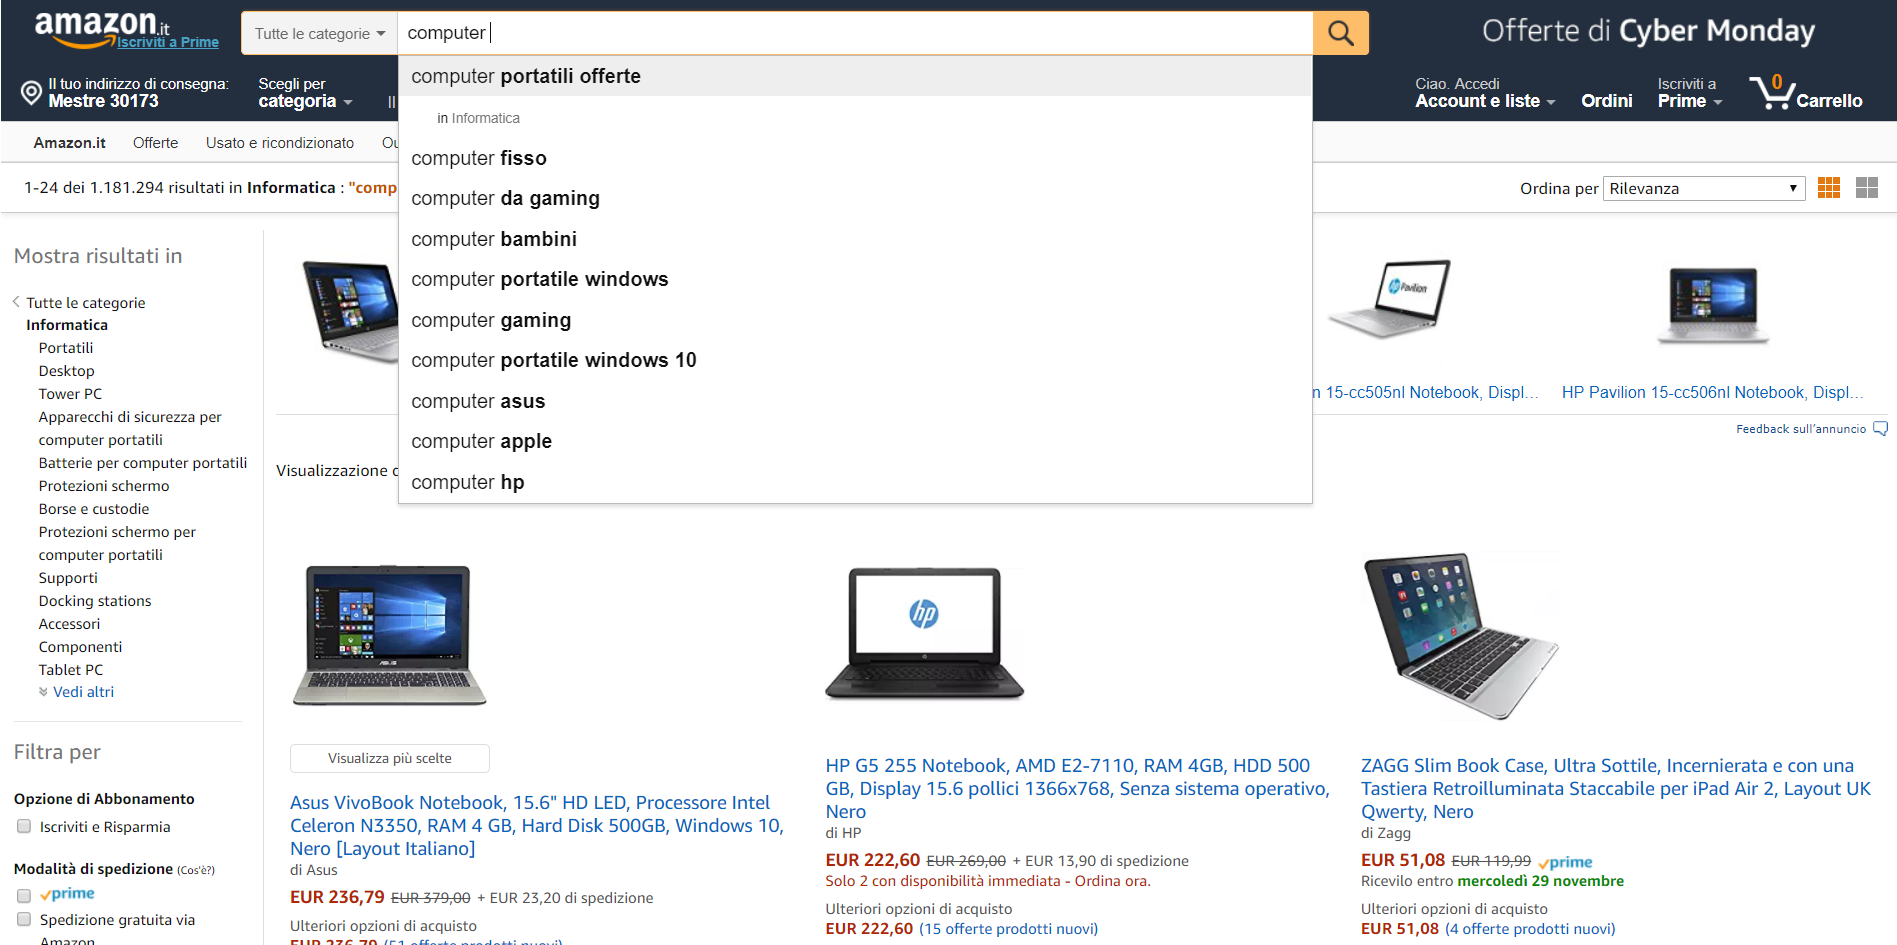
\includegraphics[width=13cm]{amazon}
			\captionof{figure}{Esempi di funzionalità di ricerca offerte dal sito di Amazon}
		\end{center}
	\end{figure}
	
	I motori di ricerca hanno assunto un ruolo fondamentale per gli utenti che navigano i siti web. Il genere di contatto che arriva da un motore di ricerca è particolarmente importante, in quanto quest'ultimo non rappresenta un utente passivo, bensì è un'entità attiva, pronta ad interagire con il suo utilizzatore. Durante una ricerca infatti, solitamente l'utente immette delle parole chiave, sperando di trovare ciò che sta cercando, con grandi aspettative derivanti dalla consultazione dei risultati. \\
	Per aiutare l'utente a trovare ciò che sta cercando, i siti web devono però fare la loro parte: è necessario infatti che vengano curati con particolare attenzione alla visibilità elementi come testi e parole chiave.\\
	Navigando i siti web, l'utente può trovare vari strumenti, messi a sua disposizione, che hanno lo scopo di aiutarlo a trovare quello che sta cercando. Tra i più importanti, troviamo:
	\begin{itemize}
		\item {\textbf{Menù}: rappresentano delle categorizzazioni delle pagine; è necessario che queste siano ben categorizzate e le voci dei menù devono essere chiaramente distinguibili l'una dall'altra. Inoltre, è fortemente sconsigliato un numero elevato di voci e di sottomenù: l'utente deve infatti poter ritrovare l'informazione che cerca in un numero molto limitato di click. Per siti che contengono una grande mole di informazioni, contenute in un gran numero di pagine, questo strumento risulta dunque essere utile ma non sufficiente, in quanto non rappresenta per l'utente uno strumento attraverso il quale trovare agevolmente i contenuti di interesse in un sito contenente un gran numero di documenti;}
		\item{\textbf{Search Box}: l’utente deve inserire in un campo di testo una o più parole chiave. Eventualmente, è possibile disporre di una ricerca avanzata, specificando uno o più filtri. Qualsiasi etichetta o filtro che permetta di inserire criteri come “cerca solo la parola esatta” oppure “escludi dalla ricerca le seguenti parole” funziona solamente se l’utente è capace di esprimere in termini logici i criteri che ha in mente. Per essere efficace, è dunque di fondamentale importanza disporre di una ricerca che sia il più possibile in grado di comprendere il linguaggio naturale dell'utente;}
		\item{\textbf{Faceted Search}: questo strumento estende l'idea dei semplici filtri di ricerca, consentendo di ricercare elementi attraverso filtri multipli, comprendendo quindi più attributi per volta nella ricerca.}
	\end{itemize}
	
	Lo scopo dello stage consisteva nell'analisi delle caratteristiche dei motori di ricerca \gls{open source} nell'ambito dei siti web di tipo informativo e, in particolare, lo studio e il confronto delle funzionalità di possibile interesse per i siti web istituzionali delle Camere di Commercio. L'obiettivo da raggiungere, consiste nel cercare di migliorare l'esperienza di navigazione, da parte degli utenti, all'interno dei siti camerali, rendendo la navigazione il più possibile efficiente, efficace e semplice. \\
	Per raggiungere questo obiettivo, in primo luogo mi è stato richiesto un approfondimento delle caratteristiche istituzionali dei siti web delle Camere di Commercio. \\
	Successivamente, l'azienda richiedeva lo studio della tecnologia \gls{Drupal} e dell'analisi delle potenzialità e specificità dei motori di ricerca \gls{Solr} e \gls{ElasticSearch}. \\
	Veniva inoltre richiesto un prototipo di un sito web in tecnologia \gls{Drupal}, con i due motori di ricerca precedentemente citati. \\
	Infine, era richiesta una relazione finale sulle potenzialità emerse nell'utilizzo dei due motori di ricerca. \\
	
	\subsection{Obiettivi posti dall'azienda}
	\label{sub:obiettivi_posti_azienda}
	
		\subsubsection{Le milestone}
		\label{subsub:milestone}
		Il Piano di Lavoro, redatto assieme al tutor aziendale che mi ha seguito durante lo stage in \nomeAzienda, prevede, tra l'altro, una serie di \gls{Milestone}; ad ognuna di esse, sono associati i prodotti sviluppati entro ogni corrispondente scadenza. Di seguito ne riporto l'elenco completo:
		
		\begin{itemize}
			\item {Fine prima settimana: Ambiente di sviluppo configurato e funzionante (n.b. per ambiente di sviluppo si intende installazione in locale di un sito web \gls{Drupal});}
			\item {Fine seconda settimana: Relazione con approfondimenti riguardanti \gls{Solr};}
			\item {Fine quarta settimana: Realizzazione prototipo di sito web in \gls{Drupal} integrato con \gls{Solr};}
			\item {Fine quinta settimana: Relazione con approfondimenti riguardanti \gls{ElasticSearch};}
			\item {Fine settima settimana: Realizzazione prototipo di sito web in \gls{Drupal} integrato con \gls{ElasticSearch};}
			\item {Fine ottava settimana: Relazione conclusiva e presentazione dell’elaborato al team di lavoro.}		
		\end{itemize}

		\begin{figure}[htbp]
			\begin{center}
				
\includegraphics[width=13cm]{milestone}
				\captionof{figure}{Milestone e metodologia di lavoro}
			\end{center}
		\end{figure}
	
		\subsubsection{Prodotti attesi}		
		L'attività di stage prevedeva la produzione di un insieme di oggetti, frutto di tale attività. Di seguito, ne è riportato l'elenco:
		
		\begin{itemize}
			\item {Documento: relazione sul motore di ricerca \gls{Solr} che riporti le caratteristiche funzionali ed architetturali della soluzione, pregi e difetti e possibile utilizzo all'interno del contesto InfoCamere;}
			\item {Documento: relazione sul motore di ricerca \gls{ElasticSearch} che riporti le caratteristiche funzionali ed architetturali della soluzione, pregi e difetti e possibile utilizzo all'interno del contesto InfoCamere;}
			\item {Documento: relazione finale di comparazione dei due motori di ricerca;}
			\item {Software: prototipo di sito web in tecnologia \gls{Drupal} che utilizza motore di ricerca \gls{Solr};}
			\item {Software: prototipo di sito web in tecnologia \gls{Drupal} che utilizza motore di ricerca \gls{ElasticSearch};}
			\item {Documento: relazione conclusiva (slide) sull'esperienza dell'uso dei prototipi, pregi e difetti nell'uso dei motori di ricerca in \gls{Drupal} e comparazioni}.
		\end{itemize}

		\subsubsection{Priorità degli obiettivi aziendali}
		\label{subsub:priorita_degli_obiettivi_aziendali}
		Gli obiettivi aziendali riguardanti lo stage possono essere suddivisi in:
		\begin{itemize}
			 \item[--] {obiettivi minimi: vincolanti in quanto richieste primarie del committente;}
			 \item[--] {obiettivi massimi: non vincolanti o strettamente necessari, ma dal riconoscibile valore aggiunto.}
	 	\end{itemize}
 	
		Di seguito, vengono riportati gli obiettivi minimi e massimi stabiliti:
		
		\begin{longtable}{| C{2cm} | C{9cm} |}
			\toprule
			\textbf{ID} & \textbf{Descrizione} \\ \hline
			\endhead	% Permette di ripetere l'intestazione nelle nuove pagine
			\midrule
			
			%%%%%	INIZIO BLOCCO FUNZIONALITA'	%%%%%
			
			\multicolumn{2}{|c|}{\cellcolor[HTML]{EFEFEF}\textbf{Obiettivi obbligatori (min) }} \\ \hline
			
				%%%%%	INIZIO BLOCCO TEST	%%%%%
				
				min01 &  Analisi dei punti di forza e debolezza dei prodotti \gls{Solr} ed \gls{ElasticSearch} \\ \hline
				
				%%%%%	FINE BLOCCO TEST	%%%%%
				
				%%%%%	INIZIO BLOCCO TEST	%%%%%
				
				min02 &  Realizzazione del prototipo in \gls{Drupal} con le funzioni minime di ricerca  \\ \hline
				
				%%%%%	FINE BLOCCO TEST	%%%%%

			%%%%%	FINE BLOCCO FUNZIONALITA'	%%%%%



			%%%%%	INIZIO BLOCCO FUNZIONALITA'	%%%%%

			\multicolumn{2}{|c|}{\cellcolor[HTML]{EFEFEF}\textbf{Obiettivi desiderabili e opzionali (max) }} \\ \hline
			
				%%%%%	INIZIO BLOCCO TEST	%%%%%
				
				max01 & Comparazione dei due motori di ricerca esaminati con altri di riferimento nel mercato \\ \hline
				
				%%%%%	FINE BLOCCO TEST	%%%%%
				
				%%%%%	INIZIO BLOCCO TEST	%%%%%
				
				max02 &  Indicazioni su possibili interventi sui siti web istituzionali per quanto riguarda la user experience di navigazione, a seguito delle potenzialità espresse dai motori di ricerca   \\ \hline
				
				%%%%%	FINE BLOCCO TEST	%%%%%
			
			%%%%%	FINE BLOCCO FUNZIONALITA'	%%%%%
			
			\bottomrule
			\caption{Obiettivi dello stage}
		\end{longtable}
		

	\subsection{Vincoli}
	
	\begin{figure}[htbp]
		\begin{center}
			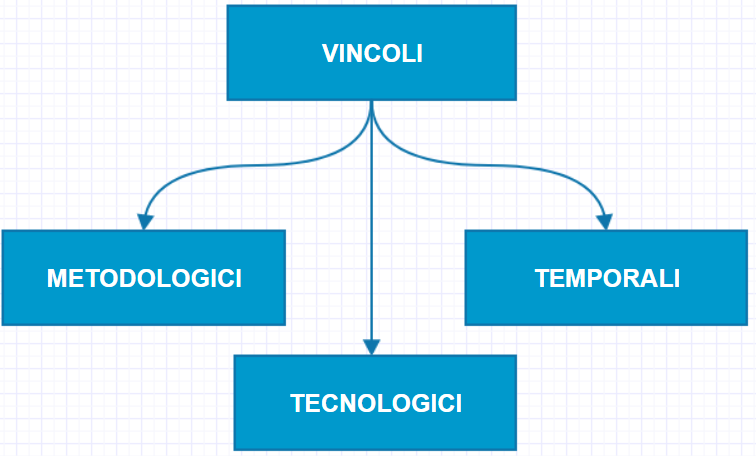
\includegraphics[height=6cm]{vincoli}
			\captionof{figure}{Tipologie di vincoli del progetto}
		\end{center}
	\end{figure}
	
		\subsubsection{Vincoli metodologici}
		In accordo con \nomeAzienda, ho svolto lo stage presso la sede di \locazioneAzienda. In questo modo, ho avuto la possibilità di confrontarmi con programmatori più esperti ed essere supportato al meglio in caso di problematiche di sviluppo e gestione del progetto; lo svolgimento dello stage in azienda aveva inoltre lo scopo di favorire l’inserimento dello stagista nell'area di sviluppo aziendale.
		Ho avuto la possibilità, a cadenza quotidiana, di discutere con il tutor aziendale per qualsiasi tipo di problema legato allo stage. Settimanalmente, abbiamo fatto il punto della situazione sullo stato del lavoro, rivedendo, quando necessario, obiettivi settimanali o eventuali miglioramenti al progetto. \\
		Nell'ultima settimana lavorativa, l'azienda ha inoltre richiesto una presentazione, esposta verbalmente e corredata da diapositive illustrative, sul lavoro operato durante lo stage e sulle relative conclusioni. \\
		Altro vincolo legato alla metodologia, riguarda invece la tipologia di installazione dell'ambiente di sviluppo. In accordo con il tutor aziendale, ho deciso di installare l'intero ambiente di sviluppo localmente, così da poter intervenire agevolmente sull'intero sistema, senza la necessità di coinvolgere i sistemisti (o comunque altri reparti aziendali), per apportare modifiche a configurazioni delle tecnologie utilizzate, in modo tale da velocizzare i tempi di intervento.
		
		\subsubsection{Vincoli tecnologici}
		Per la gestione di versione dei prodotti dello stage, InfoCamere mi ha predisposto un repository \gls{Git}, nel quale ho versionato le varie istanze dei siti \gls{Drupal} creati, assieme ai relativi \gls{Dump} dei database, oltre ai documenti scritti. \\
		Per quanto concerne la tecnologia di comunicazione, mi sono invece state fornite delle credenziali di accesso, per poter accedere all'intranet aziendale e al client di posta elettronica utilizzato da \nomeAzienda (\gls{Zimbra}), oltre a consentirmi l'accesso all'account del PC della postazione che mi è stata assegnata. \\
		Per la presentazione finale fatta in azienda ho invece utilizzato un template aziendale dedicato alle presentazioni, realizzato con Microsoft PowerPoint. \\
		Infine, le istanze \gls{Drupal} create su \gls{Acquia Dev Desktop 2} sono state realizzate in locale, seppur questa tecnologia fornisca la possibilità di ospitare le istanze sulla piattaforma \gls{Acquia Cloud}. Così facendo, è possibile non dipendere in alcun modo da tempistiche legate alla tipologia di un eventuale account su \gls{Acquia Cloud}. In futuro, sarà dunque possibile per l'azienda disporre liberamente delle istanze da me create.
		
		\subsubsection{Vincoli temporali}
		L'orario di lavoro era lo stesso previsto per il personale \nomeAzienda: dal Lunedì al Venerdì, con orari flessibili di un'ora dalle 08.00-09.00 alle 17.00-18.00 con un'ora di pausa pranzo. \\
		L'azienda mi ha fornito un badge per accedere ai locali aziendali e mi è stato inoltre richiesto di timbrare quotidianamente il badge per registrare gli orari di entrata e di uscita. Inoltre, a cadenza quotidiana, il tutor aziendale registrava le attività svolte, la data e apponeva infine la propria firma. \\
		Il numero complessivo di ore previsto dallo stage era pari a circa 300 ore, distribuite nell'arco di due mesi, con settimane lavorative di 40 ore ciascuna.

\section{Obiettivi personali}
Personalmente, ritengo che svolgere uno stage sia molto importante nell'odierno mercato del lavoro; questa opportunità porta infatti benefici, oltre che all'azienda, allo stagista stesso, sia dal punto di vista personale, sia da quello professionale. \\
Uno studente universitario apprende, nel corso del proprio percorso formativo scolastico, un gran numero di nozioni teoriche. Allo stesso tempo però, gli studenti hanno carenze sull'aspetto pratico del lavoro. Per poter sopperire a queste mancanze, permettendo allo studente di essere più competitivo nel mercato del lavoro, è di fondamentale importanza arricchire le conoscenze teoriche con esperienze professionali. \\
Lo stage permette allo studente di fare esperienza senza la necessità, da parte dell'azienda, di assumere personale privo di esperienza. \\
Oltre alle sopraccitate motivazioni, riporterò di seguito i motivi che mi hanno portato a scegliere, tra le tante aziende con le quali sono venuto a contatto grazie all'evento StageIT, \nomeAzienda.

\begin{itemize}
	\item {\textbf{Motivazioni professionali}: Essendo stata questa la mia prima esperienza lavorativa in un'azienda che lavora in ambito informatico, ho scelto \nomeAzienda, azienda con un gran numero di dipendenti e particolarmente strutturata, con la speranza di potermi confrontare con gente molto più esperta di me, con conoscenze più specifiche e capacità di problem solving differenti rispetto a quelle che si possono trovare nel mondo universitario. Inoltre, ho ritenuto l'argomento dello stage di particolare interesse, in grado di fornirmi abilità molto richieste nell'attuale mondo del lavoro. Oltre a tutto questo, ritengo inoltre di fondamentale importanza ampliare la mia rete di contatti con professionisti che lavorino nel mio stesso campo d'interesse, utile per eventuali consigli professionali, raccomandazioni di lavoro, o più semplicemente per avere confronti costruttivi. Infine, l'esperienza porterà certamente ad un valore aggiunto al mio curriculum.}
	
	\item {\textbf{Motivazioni economiche}: A differenza di altre aziende con cui ho avuto un contatto, \nomeAzienda offriva un rimborso spese e buoni pasto. Ritengo che questo tipo di riconoscimento da parte dell'azienda sia un modo per incentivare lo stagista a svolgere al meglio il proprio lavoro, oltre ad agevolare lo studente, aiutandolo a sostenere le spese che deve sostenere.}
	
	\item {\textbf{Motivazioni personali}: Ritengo che lo stage sia il momento adatto per capire se il lavoro che ho scelto e la strada che ho intrapreso sia realmente ciò che voglio fare nella mia vita.}
	
\end{itemize}		% Lo stage
	% !TEX root = ../../Tesi.tex

%******************************************
%	Resoconto dello stage
%******************************************

\chapter{Resoconto dello stage}
\label{cap:resoconto_dello_stage}

	\section{Individuazione dei motori di ricerca}
	\label{sec:individuazione_dei_motori_di_ricerca}
	Ad oggi, sono disponibili in rete un gran numero di motori di ricerca, sia proprietari, sia \gls{open source}. Questi mettono a disposizione funzionalità di ricerca più o meno avanzate e, a seconda di vari fattori come ad esempio la tipologia e la quantità di dati che vogliamo rendere ricercabili, possiamo optare per l'uno piuttosto che per l'altro. \\
	La scelta del motore di ricerca più adatto alle specifiche esigenze, non è questione affatto banale; molte volte esistono varie soluzioni in grado di modellare bene il problema che dobbiamo affrontare, simili tra loro, che differiscono però per alcuni aspetti chiave. \\
	Focalizzando l'attenzione sulle esigenze dettate dai siti informativi Camerali, possiamo subito applicare un primo filtro sui motori di ricerca da utilizzare: motori di ricerca proprietari \textit{vs} motori di ricerca \gls{open source}. \\
	Un motore di ricerca proprietario rappresenta indubbiamente un onere per l'azienda e, oltre a ciò, quest'ultima non ha il pieno controllo sulla destinazione finale dei dati; queste questioni non si hanno invece in un sistema \gls{open source}, nel quale il codice sorgente è liberamente modificabile e analizzabile, avendo dunque il pieno controllo sull'intero sistema. \\
	Nella \hyperref[img:confronto_SE]{figura 3.1} è presente una classifica dei motori di ricerca, aggiornata a Novembre 2017, calcolata su parametri che rappresentano la popolarità del sito (maggiori informazioni sui punteggi assegnati sono disponili al seguente indirizzo: \url{https://db-engines.com/en/ranking_definition}). Da questa tabella, notiamo come in testa alla classifica siano presenti tre motori di ricerca che hanno un ampio margine di distacco, in termini di punteggio ad essi attribuito, rispetto alle tecnologie che li precedono. Di questi, solamente i primi due (\gls{Solr} e \gls{ElasticSearch}) sono alternative \gls{open source}. \\
	Oltre a ciò, per entrambi i motori di ricerca appena citati, sono disponibili \glspl{Modulo} \gls{Drupal} che rendono possibile la semplice integrazione tra i motori di ricerca e il \gls{CMSg} di interesse. \\
	Le motivazioni appena descritte, hanno così portato alla selezione di \gls{Solr} e \gls{ElasticSearch} come motori di ricerca da studiare nell'ambito dello stage.

	\begin{figure}[htbp]
		\label{img:confronto_SE}
		\begin{center}
			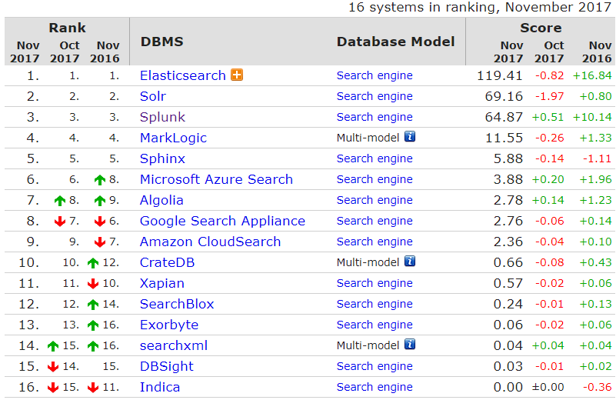
\includegraphics[width=13cm]{tabella_SE}
			\captionof{figure}{\cite{site:confronto_SE}}
		\end{center}
	\end{figure}
	
	\section{Pianificazione}
	Durante la stesura del Piano di Lavoro, assieme al tutor aziendale, ho concordato le attività principali da svolgere durante il periodo di stage, della durata di circa 300 ore, previsto dal mio Corso di Laurea. Nel documento sopracitato, sono inoltre contenute le \gls{Milestone} pianificate, così come descritto nella \hyperref[subsub:milestone]{sezione 2.2.2, sotto alla voce "Le milestone"}. \\
	Oltre al resoconto quotidiano con il tutor aziendale, al completamento di ogni attività, abbiamo fatto il punto della situazione sullo stato di avanzamento del lavoro, rivedendo e integrando, quando necessario, gli obiettivi settimanali previsti dal Piano di Lavoro. Questa modalità di operare mi ha permesso di rispettare le attività pianificate fin dall'inizio, oltre ad ampliare lo studio delle funzionalità di ricerca offerte da \gls{Drupal}, non inizialmente previste, necessarie però a fornire un quadro più dettagliato sull'intero ambito di lavoro.
	Nell'ultima settimana lavorativa, l'azienda ha inoltre richiesto una presentazione, esposta verbalmente e corredata da diapositive illustrative, sul lavoro operato durante lo stage e sulle relative conclusioni. Più nel dettaglio, nella presentazione ho esposto: scopo e motivazioni del lavoro svolto; come ho organizzato il mio lavoro; funzionalità offerte dalle tecnologie da me esaminate (di interesse per l'azienda); conclusione soggettiva su quale tecnologia sia più adatta nell'ambito dei siti camerali, con suggerimenti per migliorare le funzionalità di ricerca dei suddetti siti; benefici immediati e a lungo termine che il lavoro svolto durante lo stage ha apportato all'azienda; ulteriori ambiti da esplorare, relativamente a queste tecnologie; valutazione soggettiva, mia e del tutor aziendale, riguardo allo stage come esperienza. \\
	
	\section{I siti istituzionali delle Camere di Commercio}

		\subsection{Funzionalità di ricerca attuali}
		Quando un utente visita un sito web, è fondamentale che le informazioni in esso contenute siano facilmente trovabili dall'utente.
		A tal fine, è necessario che un sito web informativo fornisca all'utente strumenti che lo aiutino a trovare agevolmente, in pochi click, quello che sta cercando. La ricerca interna, spesso presente nei siti web, è uno di questi strumenti ed è strettamente legato ai concetti di:
		\begin{itemize}
			\item[--]{\textbf{efficienza}: il numero di azioni da che l'utente deve compiere per trovare quello che sta cercando dev'essere molto limitato; inoltre, i tempi di risposta devono essere molto brevi, quasi impercettibili agli occhi dell'utente, stando dunque nell’ordine dei msec;}
			\item[--]{\textbf{efficacia}: l’utente deve essere in grado di trovare sempre quello che cerca; lo strumento di ricerca deve comprendere quanto più possibile il linguaggio naturale con il quale l'utente comunica al sito web.}
		\end{itemize}
		
		Il fine ultimo dello stage consiste nel cercare di migliorare le funzionalità di ricerca, offerte agli utenti, degli attuali siti web istituzionali delle Camere di Commercio. \\
		Prendiamo come esempio l’attuale sito istituzionale della Camera di Commercio di Verona (\cite{site:vr_camerale}): come presentato nella \hyperref[img:conferenze]{figura 3.2}, a fronte della ricerca del termine “Conferenze”, lo strumento di ricerca interno non trova alcun risultato, a differenza invece della ricerca di “Conferenza”, presentato nella \hyperref[img:conferenza]{figura 3.3}, che produce invece alcuni risultati. Rispetto alla prima ricerca effettuata, abbiamo semplicemente cambiato la forma del termine ricercato, dal plurale della prima ricerca al singolare della seconda. \\ 
		Da questo comportamento, possiamo dunque dedurre che la ricerca venga attuata sui termini esatti, ed è ben lontana dal comprendere i linguaggi naturali.

		\begin{figure}[htbp]
			\label{img:conferenze}
			\begin{center}
				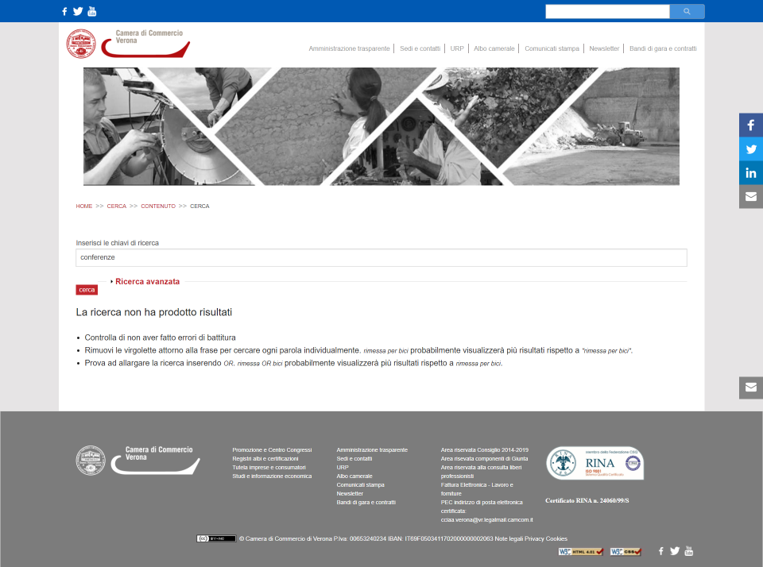
\includegraphics[width=13cm]{vr_attuale}
				\captionof{figure}{\cite{site:vr_attuale}}
			\end{center}
		\end{figure}
	
		\begin{figure}[htbp]
			\label{img:conferenza}
			\begin{center}
				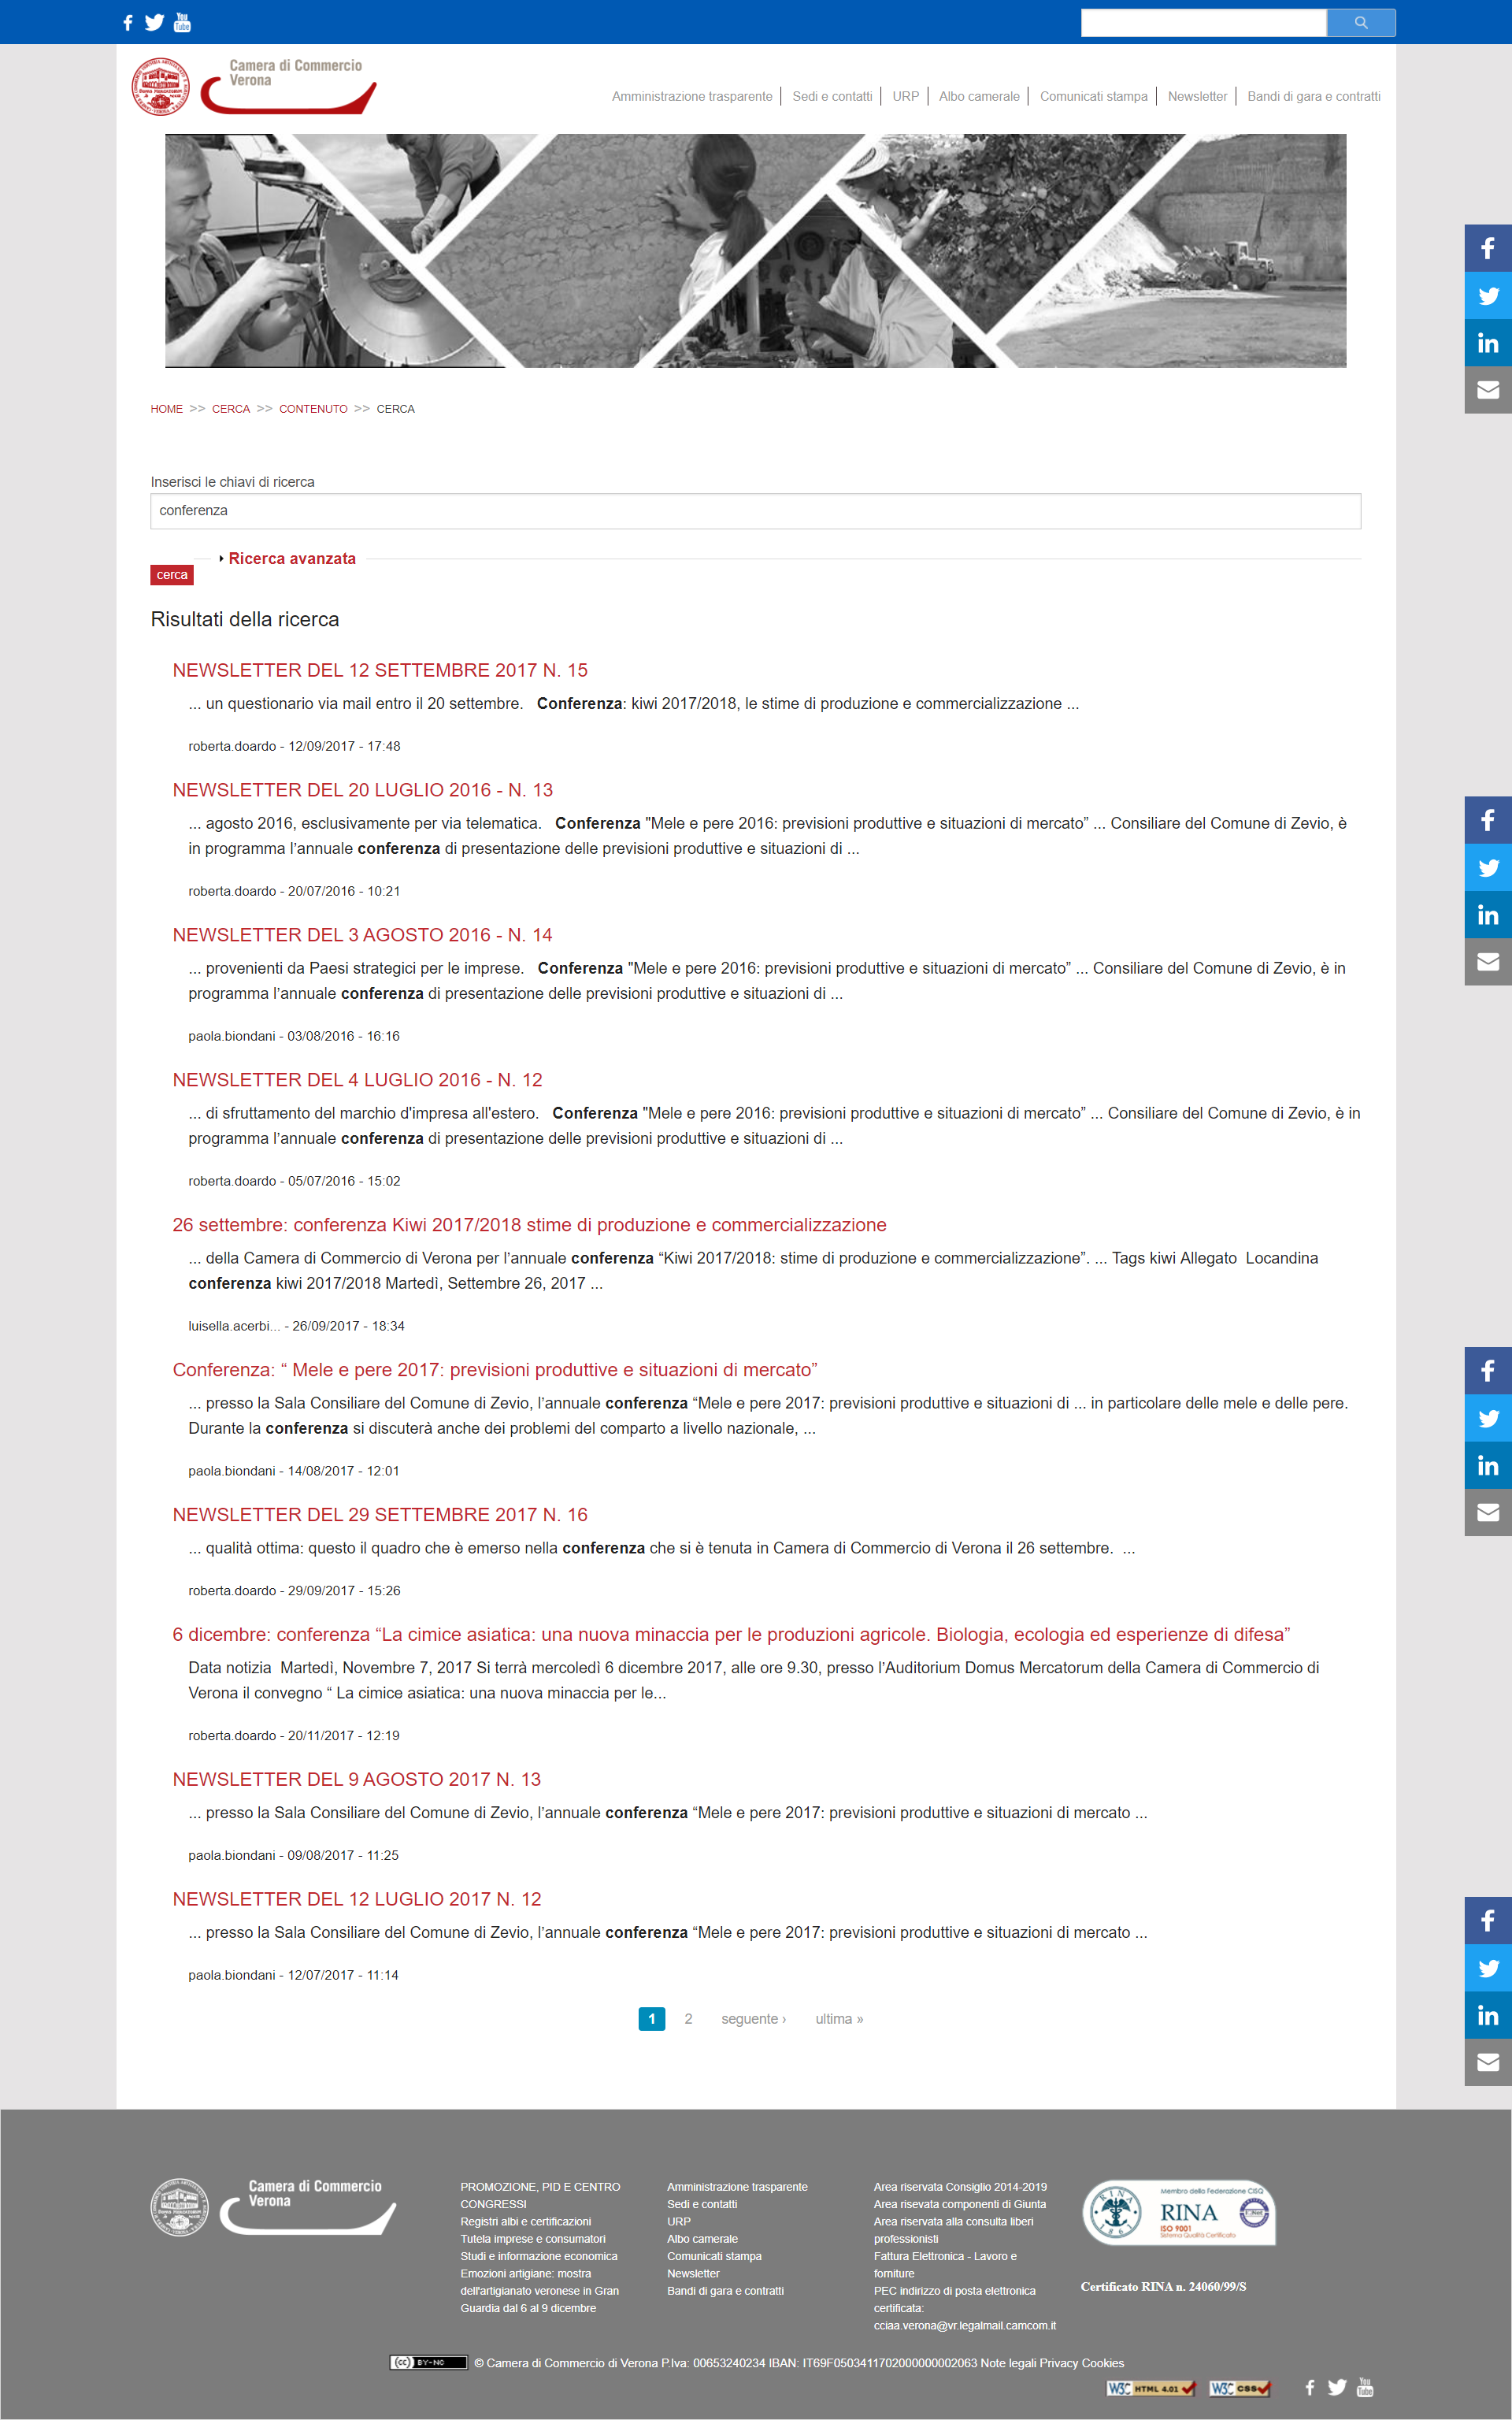
\includegraphics[width=13cm]{vr_attuale_conferenza}
				\captionof{figure}{\cite{site:vr_attuale_conferenza}}
			\end{center}
		\end{figure}
		
		\newpage
		\subsection{Possibile evoluzione}
		\label{sub:possibile_evoluzione}
		Come ho illustrato nella sezione precedente, le funzionalità di ricerca attuali sono molto limitate, ben lontane dal fornire all'utente un'esperienza di navigazione incentrato sulla ricerca, con strumenti limitati nel numero e nella qualità delle funzionalità offerte. \\
		Come possiamo dunque migliorare la ricerca nei siti informativi Camerali?
		Per perseguire questo obiettivo ambizioso, pensiamo alle funzionalità di ricerca con cui gli utenti sono soliti interagire. \\		
		Google ad esempio, mette a disposizione diverse funzionalità che aiutano l’utente ad effettuare una ricerca che produca i risultati attesi, pur gestendo un'enorme quantità di dati. I siti di e-commerce utilizzano inoltre un altro strumento molto utile ai fini di una ricerca, che consente agli utenti di filtrare le ricerche, restringendo molto rapidamente i possibili contenuti di interesse: si tratta delle facets, dette anche filtri multipli, che verranno presentati nel seguito di questo paragrafo. Alcune di queste funzionalità potrebbero essere prese come punto di partenza per migliorare la ricerca interna dei siti informativi Camerali. In particolare:
		
			\subsubsection{Completamento automatico}
			Questa caratteristica consente agli utenti di visualizzare una lista di termini suggeriti sulla base dei caratteri che hanno digitato fino a quel momento; in questo modo, viene ridotto il numero di errori di digitazione della keywords da ricercare, consentendo così ricerche più vicine a quanto pensato dagli utenti, avvicinandosi in tal modo alle loro esigenze. \\ Ulteriore vantaggio è dato dalla riduzione del tempo richiesto agli utenti per effettuare una ricerca, in quanto se questa è presente tra le keywords suggerite, l'utente può risparmiare tempo semplicemente selezionando il suggerimento offerto dal sistema, così da non dover digitare interamente i termini da ricercare, rendendo in tal modo la ricerca maggiormente efficiente in termini temporali.
			\begin{figure}[htbp]
				\begin{center}
					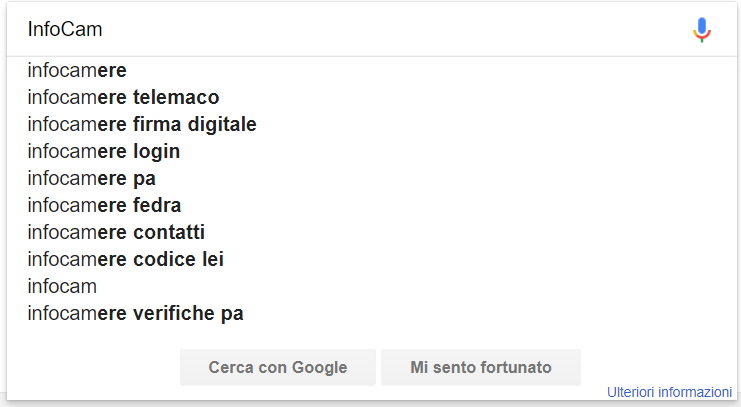
\includegraphics[width=7cm]{completamento_automatico}
					\captionof{figure}{Funzionalità di completamento automatico di Google}
				\end{center}
			\end{figure}
		
			\subsubsection{Paginazione e ordinamento}
			La funzionalità di paginazione permette di rendere le ricerche più rapide, restituendo un sottoinsieme dei risultati di ricerca.
			L'ordinamento consente invece di ordinare i risultati restituiti a seguito di una ricerca, sulla base di specifiche caratteristiche dei documenti indicizzati.
			
			\subsubsection{Controllo ortografico}
			Funzionalità indispensabile per comprendere quanto più possibile il linguaggio naturale con il quale l'utente comunica; può essere gestito come:
			\begin{itemize}
				\item {Correzione automatica: viene eseguito automaticamente il controllo ortografico dei termini ricercati, sulla base del fatto che il termine contenente errori ortografici sia indicizzato;}
				\item {"Did you mean...?": vengono suggerite ricerche che potrebbero produrre risultati migliori; l'utente visualizzerà l'elenco di questi suggermenti.}
			\end{itemize}

			\begin{figure}[htbp]
				\begin{center}
					
\includegraphics[width=7cm]{did_you_mean}
					\captionof{figure}{Esempio funzionalità "Did you mean...?" in Google}
				\end{center}
			\end{figure}

			\subsubsection{Evidenziamento delle parole ricercate nei risultati}
			Quando vengono ricercati documenti che contengono una quantità significativa di testo, è bene fornire all'utente la possibilità di visualizzare sezioni specifiche di ogni documento, mettendo in risalto le sezioni dei risultati di ricerca contenenti i termini ricercati dagli utenti.
			
			\begin{figure}[htbp]
				\begin{center}
					
\includegraphics[width=7cm]{highlighting}
					\captionof{figure}{Esempio funzionalità di evidenziamento, nei risultati, del termine ricercato}
				\end{center}
			\end{figure}
		
			\subsubsection{Ricerca su file}
			L'utente può trovare, tra i risultati della ricerca che ha effettuato, documenti in vari formati (PDF, doc, ecc...) che contengono le keywords ricercate. Questa funzionalità risulta essere di particolare interesse nell'ambito dei siti informativi Camerali, data la grande mole di dati contenuti in documenti memorizzati in vari formati (prevalentemente PDF).
			
			\begin{figure}[htbp]
				\begin{center}
					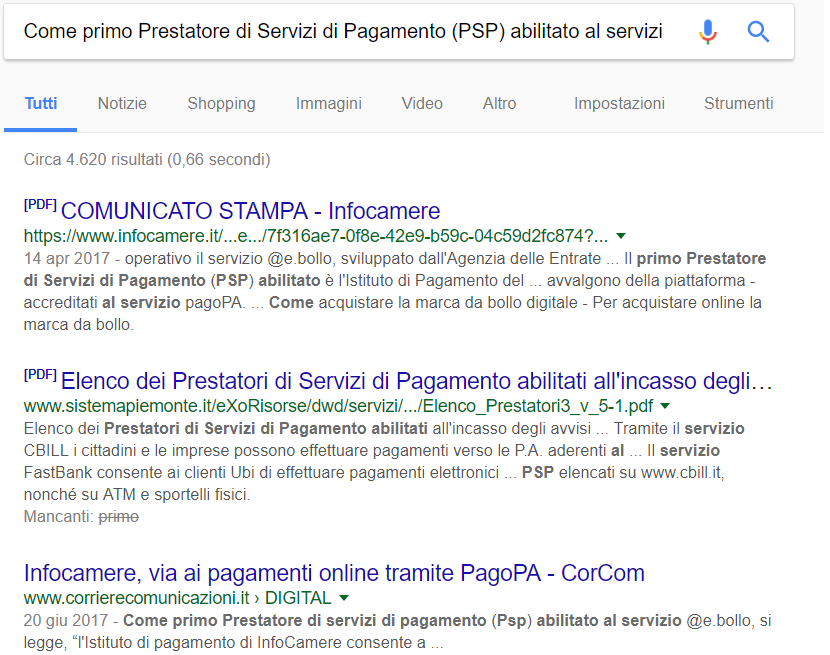
\includegraphics[width=7cm]{ricerca_su_file}
					\captionof{figure}{Esempio funzionalità di ricerca su file offerto da Google}
				\end{center}
			\end{figure}
		
			\subsubsection{Facets}
			Prevalentemente utilizzati nei siti di e-commerce, l'utilizzo di questa funzionalità permette di fornire agli utenti strumenti utili a raffinare le proprie ricerche, ricorrendo a una serie di filtri che consentono di ridurre rapidamente il numero dei risultati di ricerca, selezionando le caratteristiche di interesse di quanto ricercato. In questo modo, l'utente è in grado di costruire il proprio percorso di ricerca, consentendogli di effettuare ricerche più flessibili, che lo aiutino a trovare ciò che sta cercando con poche azioni. \\
			Al fine di rendere efficaci i filtri multipli, è di fondamentale importanza che i contenuti siano ben categorizzati, così da permettere all'utente di trovare quanto cercato.
			
			\begin{figure}[htbp]
				\begin{center}
					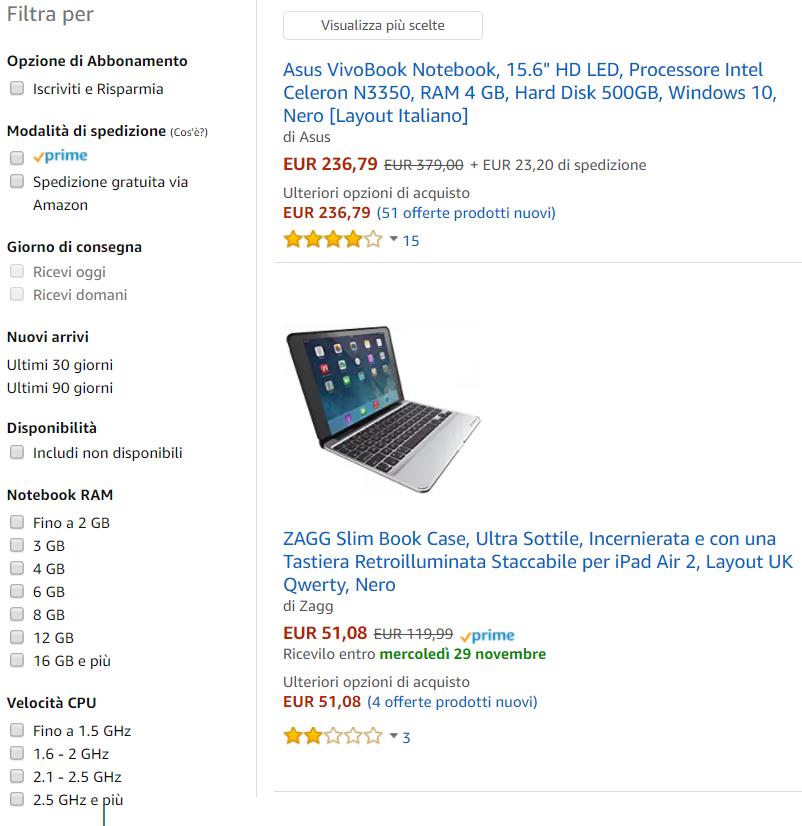
\includegraphics[width=7cm]{facets}
					\captionof{figure}{Esempio funzionalità di filtri multipli (facets) presente su Amazon}
				\end{center}
			\end{figure}
		
			\subsubsection{Importare le funzionalità nei siti informativi Camerali}
			Con l'obiettivo di migliorare la ricerca all'interno dei siti web informativi delle Camere di Commercio, in accordo con il tutor aziendale, abbiamo scelto di concentrare lo studio delle funzionalità offerte dai motori di ricerca oggetto di analisi, principalmente sugli strumenti appena presentati. \\
			Quello a cui vogliamo ambire, è presentato in un prototipo da me creato durante lo stage, contenente alcune delle funzionalità sopra esposte; un esempio è visibile nella \hyperref[img:evoluzioneVR]{Figura 3.9}. \\
			Il prototipo è stato creato con i medesimi dati contenuti nell'attuale sito web informativo della Camera di Commercio di Verona. Il termine ricercato presentato nella figura, è lo stesso della \hyperref[img:conferenze]{ricerca effettuata nell'attuale sito istituzionale camerale di Verona}, ovvero "Conferenze", che, come ho descritto in precedenza, non aveva prodotto alcun risultato. Notiamo invece che nel prototipo realizzato, la ricerca del medesimo termine sui medesimi contenuti ha invece prodotto alcuni risultati. Questo è stato possibile migliorando la funzionalità di ricerca, rendendola più flessibile e aumentando la capacità di comprensione del linguaggio naturale della stessa.

			\label{img:evoluzioneVR}
			\begin{figure}[htbp]
				\begin{center}
					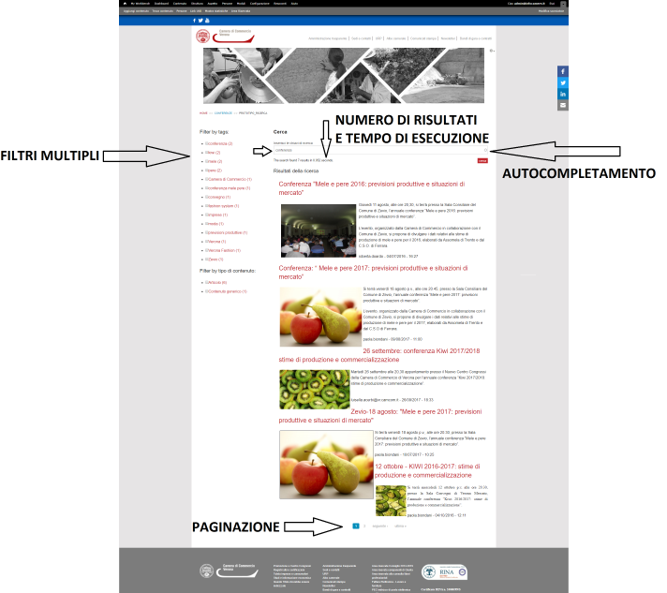
\includegraphics[width=13cm]{vr_futura}
					\captionof{figure}{Possibile evoluzione, mediante aggiunta di funzionalità di ricerca, del sito informativo Camerale di Verona}
				\end{center}
			\end{figure}

	\section{Ricerca nativa Drupal}

		\subsection{Introduzione a Drupal}
		Per giungere allo studio delle funzionalità offerte dai motori di ricerca \gls{Solr} ed \gls{ElasticSearch}, mi sono prima confrontato con \gls{Drupal}, tecnologia attualmente utilizzata da \nomeAzienda per la creazione dei siti web informativi Camerali. Come viene presentato nella \hyperref[img:cciaa_drupal]{Figura 3.10}, tale tecnologia è l'ambiente con il quale gli utenti comunicano. Le funzionalità di ricerca offerte dai siti creati in \gls{Drupal} possono servirsi di moduli di ricerca internamente presenti all'ambiente, oppure utilizzare connettori in grado di usufruire di motori di ricerca esterni, come possono essere \gls{Solr} ed \gls{ElasticSearch}.
		
		\label{img:cciaa_drupal}
		\begin{figure}[htbp]
			\begin{center}
				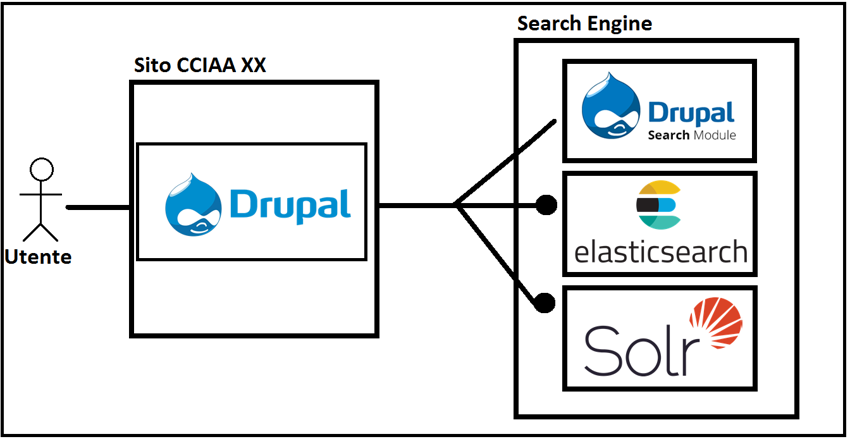
\includegraphics[width=13cm]{cciaa_drupal}
				\captionof{figure}{Utilizzo del motore da parte di un sito Camerale}
			\end{center}
		\end{figure}
	
		Facciamo un passo indietro, e chiediamoci: cos'è Drupal?
		Questa tecnologia è un \gls{CMSg} che permette di creare siti web di vario tipo, rilasciato sotto licenza \gls{open source} e interamente sviluppato in \gls{PHP}, supportando nativamente \gls{MySQL} come base di dati. Inoltre, rappresenta un'applicazione completamente web based, potendo dunque essere utilizzata attraverso un semplice browser. \\		
		L'ambiente \gls{Drupal} mette a disposizione \glspl{Modulo} che consentono di aggiungere funzionalità di ricerca al sito che stiamo realizzando. In particolare, è disponibile una \hyperref[cap:drupalSearch]{ricerca di base e avanzata} e una \hyperref[cap:drupalSearchAPI]{ricerca che sfrutta il modulo Search API offerto da Drupal}, che differiscono tra loro essenzialmente per le funzionalità offerte. Per ognuna di esse, ne ho analizzato le principali caratteristiche, focalizzando l'attenzione sulle funzionalità di possibile interesse per i siti web informativi camerali.
		
			\subsubsection {Scelta della versione Drupal}
			Sono disponibili diverse versioni \gls{Drupal}. Quella utilizzata per tutte le istanze create è la versione 7.56. La scelta deriva dalla volontà di partire da una istanza basilare, contenente solamente i moduli appartenenti al core di questa tecnologia. Esiste inoltre una versione più avanzata, ovvero Drupal 8.x; il motivo per cui la scelta è ricaduta sulla versione 7.x è dato dalla mancanza di moduli aggiornati alla versione 8. Per questo motivo, viene dunque utilizzata una versione più vecchia, della quale sono però presenti un maggior numero di \glspl{Modulo}, oltre ad essere la versione attualmente utilizzata in azienda.
		
		\subsection{Ricerca di base e avanzata}

		\begin{figure}[htbp]
			\begin{center}
				
\includegraphics[width=7cm]{drupal_search_module}
				\captionof{figure}{Ricerca di base e avanzata, offerta dei moduli presenti nel core di Drupal}
			\end{center}
		\end{figure}
	
			\subsubsection{Modalità di operare}
			Per questa tipologia di ricerca, come per tutte quelle che seguono in questo capitolo, ho proceduto innanzitutto alla creazione di una nuova istanza \gls{Drupal}, dedicata alla tipologia di ricerca in esame. Dopo una iniziale configurazione dell'ambiente, ricercando e installando i moduli che mi fornissero le funzionalità di maggior interesse, ho proceduto allo studio delle funzionalità offerte. \\
			Di seguito, riporto le conclusioni emerse dallo studio della ricerca di base e avanzata, resi disponibili dai moduli nativamente contenuti nel core di \gls{Drupal}.

			\subsubsection{Considerazioni sulla ricerca di base e avanzata}
			Una ricerca esaustiva prodotta con questa tecnologia richiede che l'utente conosca esattamente quello che sta ricercando; i contenuti hanno inoltre la necessità di essere fortemente atomizzati e specifici, mediante l'utilizzo di termini significativi, in modo tale da poter essere trovati dall'utente. \\
			Nei siti informativi Camerali, questo limite può essere mitigato ricorrendo all'utilizzo di \gls{Tag}, attraverso la creazione di \glspl{Tassonomia}, in modo da consentire all'utente una navigazione dei contenuti per tag. Così facendo, l'utente dovrà comunque conoscere con esattezza i termini chiave da ricercare e i contenuti dovranno essere etichettati in maniera corretta e specifica per i contenuti. Tutto ciò, porterebbe ad un rapido aumento del numero di tag, rendendo il sistema poco efficiente e fruibile. \\
			Un'ulteriore difficoltà che incontra questo approccio è da ricercarsi nel carico di lavoro che il server sul quale il sito viene ospitato è in grado di gestire. Non essendoci infatti la possibilità di definire engine di ricerca esterni all'ambiente \gls{Drupal}, avendo quindi un database comune, utilizzato anche per effettuare le ricerche, un elevato quantitativo di interrogazioni al database potrebbe causare ritardi significativi o addirittura interruzioni dei servizi offerti dal sito. \\
			Le ricerche di base e avanzata risultano dunque essere primitive, non adatte all'attuale stato di avanzamento tecnologico che si può osservare in vari siti informativi e non adatte a gestire siti di grandi dimensioni, dato lo scarso livello di performance e funzionalità offerte.
		
		\subsection{Ricerca con Search API}
		
			\subsubsection{Modalità di operare}
			Per prima cosa, ho proceduto alla creazione di un'istanza \gls{Drupal} dedicata alla ricerca di con \gls{Search API}.
			Oltre all'installazione di moduli di utilità, non significativi ai fini della ricerca ma che semplificano l'utilizzo dell'intero ambiente di sviluppo, ho installato il modulo \gls{Search API}. \\
			Tale modulo fornisce un \gls{Framework} per creare agevolmente ricerche nell'ambiente \gls{Drupal}, utilizzando qualunque tipologia di motore di ricerca. Prima di arrivare a studiare l'integrazione di questo modulo con i motori \gls{Solr} e \gls{ElasticSearch}, ho sfruttato una ricerca che utilizzasse un \gls{Server} interno all'ambiente \gls{Drupal}, ritrovando ciò nel \gls{Modulo} \gls{Search API Database}.
			Di seguito, riporto le conclusioni emerse dallo studio della ricerca con \gls{Search API} che sfrutta il modulo \gls{Search API Database}.
			
			\subsubsection{Considerazioni sulla ricerca con Search API Database}
			La ricerca \gls{Search API} che utilizza \gls{Search API Database} come \gls{Server} di ricerca, permette di effettuare ricerche in modo molto più flessibile rispetto a quanto offerto dalle ricerche di base e avanzata.
			Questa tecnologia permette un certo grado di complessità nelle stringhe ricercate, offrendo funzionalità molto più adatte alle aspettative degli utenti che navigano il web ai nostri giorni. \\
			\gls{Search API} non supporta tutte le funzionalità offerte dalla ricerca di base e avanzata: in particolare non sono presenti le funzionalità di ricerca che utilizzano clausole condizionali (and, or, not, ...). \\
			Le funzionalità aggiuntive, non presenti nei \glspl{Modulo} contenuti nel core di \gls{Drupal}, consentono però di eseguire ricerche più intelligenti, che aiutano l'utente a trovare contenuti ricercando termini anche non completamente esatti o incompleti. \\
			Le ricerche risultano essere molto più user friendly rispetto a quelle rese disponibili dalla ricerca di base e avanzata, evidenziando un importante passo avanti, date le funzionalità offerte, permettendo agli utenti un margine di flessibilità nei termini ricercati, che non devono dunque conoscere esattamente il termine o il concetto che stanno ricercando. \\
			Il carico di lavoro richiesto dal server sul quale il sito viene ospitato rappresenta un punto critico di questa tecnologia di ricerca: così come per la ricerca di base e avanzata, la ricerca \gls{Search API} che utilizza \gls{Search API Database}, continua a lavorare con un unico database comune, utilizzato anche per effettuare ricerche. Un elevato quantitativo di richieste e l'impossibilità di esternalizzare l'engine di ricerca su macchine che lavorino in modo concorrente potrebbe dunque compromettere i tempi di attesa per ottenere i risultati di ricerca, che diventano critici su siti di grandi dimensioni e con un gran numero di contenuti.

		\subsection{Considerazioni di Drupal nativo}
		la ricerca nativa di \gls{Drupal} permette un gran numero di funzionalità che potrebbero essere di interesse per i siti Camerali. Ulteriori \glspl{Modulo} amplificano inoltre le funzionalità possibilmente utili disponibili mediante l'utilizzo di questa tipologia di ricerca, permettendo funzionalità di completamento automatico, paginazione delle ricerche e ordinamento dei risultati di ricerca secondo filtri prestabiliti, "Did you mean...?", evidenziamento dei termini ricercati nei risultati, utilizzo di \glspl{Modulo} per implementare le facets (=filtri multipli), creazione di più \gls{Index} di ricerca e possibilità di effettuare ricerche nei contenuti testuali di alcuni tipi di files (PDF, Word, ecc...). \\
		Questa tecnologia consente dunque di effettuare ricerche con un certo grado di complessità, offrendo funzionalità molto più adatte alle aspettative degli utenti che navigano il web nei nostri giorni. \\
		La ricerca sulle \gls{Stem Words} rappresenta un possibile punto debole di questa tecnologia, non essendo attualmente disponibile un modulo nella versione 7.x per la lingua italiana.\\
		Il carico di lavoro richiesto dal server sul quale il sito viene ospitato rappresenta un punto critico di questa tecnologia. In entrambe le tipologie di ricerca presentate per la ricerca nativa \gls{Drupal}, è presente un unico database comune. Un elevato quantitativo di richieste, unito all'impossibilità di esternalizzare l'engine di ricerca su macchine che lavorino in modo concorrente potrebbe dunque compromettere i tempi di attesa per ottenere i risultati di ricerca, che diventano critici su siti di grandi dimensioni e con un gran numero di contenuti.

	\section{Ricerca con Solr}

		\subsection{Introduzione a Solr}
		
		\begin{figure}[htbp]
			\begin{center}
				
\includegraphics[width=7cm]{logo_solr}
				\captionof{figure}{Logo ricerca Solr}
			\end{center}
		\end{figure}
	
		\gls{Solr} rappresenta una piattaforma di ricerca \gls{open source}, scritta in \gls{Java}, che viene eseguita come server di ricerca full text indipendente, all'interno di un contenitore \gls{Servlet}. Utilizza \gls{Java Lucene} come libreria per la ricerca e l'indicizzazione full text e mette a disposizione chiamate \gls{REST}, supportando vari formati tra i quali \gls{JSONg} e \gls{XMLg}, rendendo la comunicazione semplice e versatile. \\ Nonostante sia scritto in \gls{Java}, non è necessaria una conoscenza di tale linguaggio per utilizzare questa tecnologia; è inoltre possibile estendere la libreria di ricerca: in questo caso la conoscenza di \gls{Java} risulterebbe, ovviamente, fondamentale. \\
		Questa tecnologia mette a disposizione un gran numero di funzionalità che aiutano l'utilizzatore ad eseguire ricerche semplici e intuitive ma potenti al tempo stesso.
		
		\subsection{Principali funzionalità di ricerca}
		
			\subsubsection{Modalità di operare}
			Dopo uno studio iniziale riguardante l'architettura ad alto livello della tecnologia, ho proceduto alla creazione e alla configurazione di una nuova istanza \gls{Solr}; la versione che ho utilizzato è la 5.5.4. Successivamente, ne ho studiato le funzionalità di ricerca più significative offerte dalla tecnologia in esame, prestando attenzione alla sua integrazione con l'ambiente \gls{Drupal}.
			
			\subsubsection{Architettura ad alto livello}
			\label{solr:architettura_ad_alto_livello}
			Per lo studio dell'architettura ad alto livello di questa tecnologia, mi sono servito di letteratura e materiale trovato in rete. Con le fonti trovate, ho individuato le seguenti componenti che vanno a comporre l'architettura di massima di \gls{Solr}, presentate di seguito.
			
			\begin{itemize}
				\label{solr:request_handler}
				\item {\textbf{Request Handler:} Le richieste che arrivano al sistema \gls{Solr} vengono processate da questa componente e possono essere di interrogazione o di aggiornamento dell'\gls{Index}; }
				
				\item{\textbf{Search Components:} Rappresenta l'insieme delle funzionalità di ricerca (faceting, highlighting, more like this, ecc...) offerte da Apache Solr. Le singole componenti di ricerca (search component) si registrano come gestori di ricerca (search handlers). E' inoltre possibile registrare più componenti in un singolo search handler;}
				
				\label{solr:query_parser}
				\item{\textbf{Query Parser:} Il \gls{Parser} di Apache Solr analizza le query passate a \gls{Solr}, verificandone la correttezza sintattica. Successivamente, traduce le interrogazioni in un formato comprensibile a \gls{Java Lucene};}
				
				\item{\textbf{Response Writer:} Componente che si occupa della generazione dell'output a seguito delle interrogazioni eseguite. Vengono supportati vari formati, tra cui \gls{XMLg}, \gls{JSONg}, ecc...;}
				
				\label{solr:analyzer_tokenizer}
				\item{\textbf{Analyzer/tokenizer:} Apache Solr analizza il contenuto e lo divide in \glspl{Token} che verranno successivamente inviati a \gls{Java Lucene}. Un Analyzer esamina il testo dei campi del contenuto e genera un flusso di token. Successivamente, questo flusso di token viene suddiviso in singoli token da un \gls{Tokenizer};}
				
				\item{\textbf{Update Request Processor:} Ogni richiesta di aggiornamento inviata ad Apache Solr passa attraverso una serie di processi, responsabili delle modifiche (eliminazioni, aggiunte di campi, ecc...), che insieme vengono definiti update request processor.}
				
			\end{itemize}
			
			\begin{figure}[p]
				\makebox[\linewidth]{
					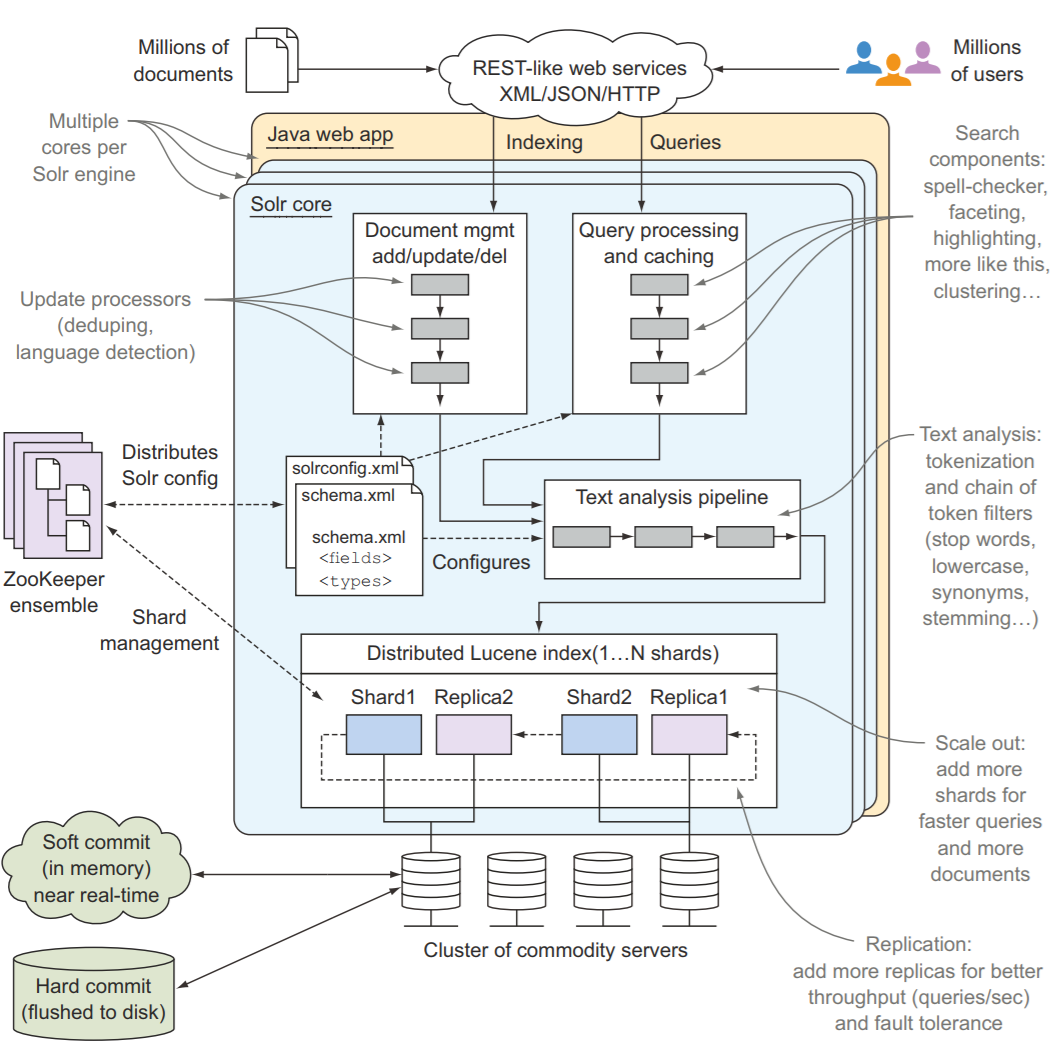
\includegraphics[width=1.3\linewidth]{solr_architettura}
				}
				\caption{Diagramma delle componenti principali di Solr}
			\end{figure}
			
			\subsubsection{Considerazioni sulla ricerca Solr}
			Per ogni tipologia di funzionalità di interesse per i siti informativi Camerali, ho proceduto alla configurazione delle componenti in modo tale da creare esempi funzionanti che supportassero la funzionalità in esame. In particolare, ho potuto constatare che tutte le funzionalità di possibile interesse per \nomeAzienda, presentate in \hyperref[sub:possibile_evoluzione]{3.3.2}, vengono offerte e supportate da \gls{Solr}. \\
			Lo step successivo, consisteva nel verificare se tali funzionalità continuavano ad essere supportate integrando questo motore di ricerca con l'ambiente \gls{Drupal}, in quanto quest'ultimo avrebbe potuto agire da collo di bottiglia.

		\subsection{Integrazione con Drupal}
		Le versioni di \gls{Drupal} (7.56) e di \gls{Solr} (5.5.4) utilizzate permettono l'integrazione di queste due tecnologie in due differenti modalità, presentate di seguito.
		
			\subsubsection{Apache Solr}
			Apache Solr permette di integrare il motore di ricerca \gls{Solr} con l'ambiente \gls{Drupal} mediante utilizzo di un apposito \gls{Modulo}, denominato "Apache Solr". Questo modulo mette in comunicazione il modulo di ricerca "Search" offerto dal core di \gls{Drupal} con il motore di ricerca. \\
			Dopo aver creato e configurato un'apposita istanza \gls{Drupal} che utilizzasse il suddetto modulo, ho potuto constatare che, pur utilizzando un potente motore di ricerca, non vengono supportate alcune delle funzionalità di possibile interesse per i siti Camerali, data l'assenza di \glspl{Modulo} necessari all'integrazione della ricerca di base e avanzata con \gls{Solr}. In particolare, un'istanza \gls{Drupal} che utilizzi il modulo "Apache Solr" non permette l'utilizzo dei filtri multipli nè la creazione di più indici, utili per gestire tipologie di ricerca che differiscano per tipo di documento/entità ricercata, all'interno di un sito.
			
			\subsubsection{Search API Solr}
			Search API Solr permette di integrare il motore di ricerca \gls{Solr} con l'ambiente \gls{Drupal} utilizzando il modulo "Search API Solr", che funge da connettore tra le due tecnologie, mettendo in comunicazione il modulo di ricerca \gls{Search API} con il motore di ricerca. \\
			Dopo aver creato e configurato un'apposita istanza \gls{Drupal} che utilizzasse il suddetto modulo, ho avuto modo di vedere che tutte le funzionalità di possibile interesse per i siti Camerali vengono ben supportate da questa tipologia di integrazione, risultando essere lo strumento di maggior interesse tra tutti quelli presentati fino ad ora.
	
	\section{Ricerca con ElasticSearch}
	
		\subsection{Introduzione a ElasticSearch}
		
		\begin{figure}[htbp]
			\begin{center}
				
\includegraphics[width=7cm]{logo_elasticSearch}
				\captionof{figure}{Logo ricerca ElasticSearch}
			\end{center}
		\end{figure}
		
		\gls{ElasticSearch} è una piattaforma di ricerca \gls{open source}, con capacità di ricerca full text. E' un server di ricerca basato su \gls{Java Lucene} e supporta architetture distribuite. Tutte le funzionalità sono nativamente esposte tramite interfaccia \gls{RESTful}; le informazioni sono invece gestite come documenti \gls{JSONg}. \\
		Questa tecnologia è divenuta molto popolare nell'ambito Big Data, negli ambienti enterprise e nel settore del cloud computing, date le funzionalità di ricerca, analisi e visualizzazione dei contenuti nei documenti \gls{JSONg}, con interrogazioni che avvengono quasi in tempo reale. \\
		Assieme a \gls{Kibana} e \gls{Logstash}, produce una soluzione integrata, in grado di gestire grandi quantità di log in una forma centralizzata, facilmente ricercabile e che usi un'interfaccia grafica intuitiva; questi tre software vanno a produrre quello che viene definito "Elastic Stack" (ELK stack).

		\subsection{Principali funzionalità di ricerca}
		
			\subsubsection{Modalità di operare}
			Dopo uno studio iniziale riguardante l'architettura ad alto livello della tecnologia, ho proceduto alla creazione e alla configurazione di una nuova istanza \gls{ElasticSearch}; la versione che ho utilizzato è la 5.6.4. Per semplificare l'utilizzo di questo strumento, ho utilizzato \gls{Cerebro}, un tool che consente di avere una visione grafica degli indici di ricerca creati in \gls{ElasticSearch} e che fornisce uno strumento per effettuare, in modo semplice, chiamate \gls{REST}, in modo tale da poter comunicare con il server di ricerca.
			Successivamente, ne ho studiato le funzionalità di ricerca più significative offerte dalla tecnologia in esame, prestando attenzione alla sua integrazione con l'ambiente \gls{Drupal}.
			
			\subsubsection{Architettura ad alto livello}
			L'architettura di \gls{ElasticSearch} pone le sue fondamenta nel linguaggio \gls{Java} e consente l'esecuzione di ricerche full text all'interno di un contenitore \gls{Servlet}. Così come accade per \gls{Solr}, \gls{ElasticSearch} utilizza \gls{Java Lucene} come libreria per la ricerca. Qui le comunicazioni passano da un'interfaccia di tipo \gls{RESTful} e le informazioni vengono gestite come documenti \gls{JSONg}.\\
			Una delle caratteristiche importanti di \gls{ElasticSearch} riguardanti la gestione degli event log, è quella di essere priva di uno schema, rendendo in tal modo possibile, a seguito dell'inserimento di un qualsiasi documento in formato \gls{JSONg}, l'indicizzazione di tutti i suoi campi, consentendo così di poter essere utilizzati per eseguire query di ricerca. \\
			Nella letteratura e nel materiale ricercato in rete, non ho trovato una spiegazione chiara ed esaustiva sull'architettura ad alto livello di questa tecnologia. Assieme al tutor, partendo dall'architettura studiata per \gls{Solr}, abbiamo dunque cercato di disegnare un'architettura di massima di questo motore di ricerca. Le principali componenti che abbiamo individuato sono le stesse di quelle presenti per \gls{Solr}, \hyperref[solr:architettura_ad_alto_livello]{presentate in precedenza in questo capitolo}.

			\begin{figure}[p]
				\makebox[\linewidth]{
					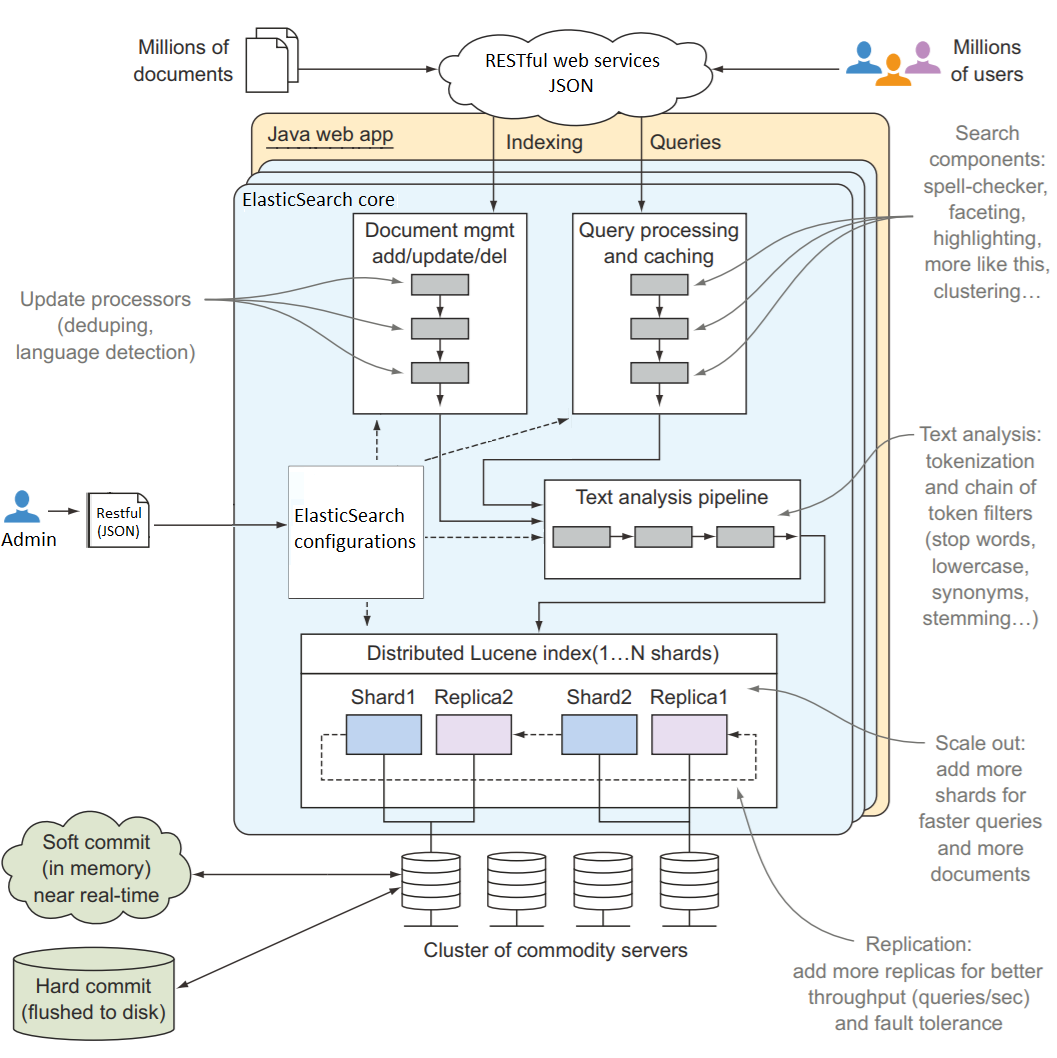
\includegraphics[width=1.3\linewidth]{elasticsearch_architettura}
				}
				\caption{Diagramma delle componenti principali di ElasticSearch}
			\end{figure}
			
			\subsubsection{Considerazioni sulla ricerca ElasticSearch}
			Così come ho operato per lo studio di \gls{Solr}, anche per \gls{ElasticSearch}, per ogni tipologia di funzionalità di interesse per i siti informativi Camerali, ho proceduto alla configurazione delle componenti in modo tale da creare esempi funzionanti che supportassero la funzionalità in esame. Anche in questo caso, ho potuto constatare che tutte le funzionalità di possibile interesse per \nomeAzienda, presentate in \hyperref[sub:possibile_evoluzione]{3.3.2}, sono ben supportate da \gls{ElasticSearch}. \\
			Lo step successivo, consisteva nel verificare se tali funzionalità continuavano ad essere supportate integrando questo motore di ricerca con l'ambiente \gls{Drupal}, in quanto quest'ultimo avrebbe potuto agire da collo di bottiglia.
		
		\subsection{Integrazione con Drupal}
		Le versioni di \gls{Drupal} (7.56) e di \gls{ElasticSearch} (5.6.4) utilizzate permettono l'integrazione di queste due tecnologie in una sola modalità, di seguito presentata.
		
			\subsubsection{Search API ElasticSearch}
			Search API Solr permette di integrare il motore di ricerca \gls{Solr} con l'ambiente \gls{Drupal} utilizzando il modulo "Search API ElasticSearch", che funge da connettore tra le due tecnologie, mettendo in comunicazione il modulo di ricerca \gls{Search API} con il server di ricerca in esame. \\
			Dopo aver creato e configurato un'apposita istanza \gls{Drupal} che utilizzasse il suddetto modulo, ho avuto modo di vedere che tutte le funzionalità di possibile interesse per i siti Camerali, risultando essere dunque una valida alternativa a quanto offerto dalla ricerca con Search API Solr.

	\section{Considerazioni finali sui motori di ricerca esaminati}
	Dallo studio sulle funzionalità supportate dalle tecnologie di ricerca esaminate, ho prodotto una tabella riassuntiva, riportata di seguito, che illustra le funzionalità rese disponibili dalle varie tecnologie. E' bene sottolineare che tecnologie diverse possono supportare più o meno bene le singole funzionalità; un esempio per comprendere meglio questo concetto emerge dalla funzionalità di ricerca sui files: il numero di tipologie di file supportati è molto maggiore negli ambienti che utilizzano i motori di ricerca \gls{Solr} e \gls{ElasticSearch}, a differenza invece della ricerca nativa, in grado di supportare un insieme molto limitato di estensioni, tra i quali è però presente il formato PDF, che risulta essere quello di maggior interesse per l'azienda. \\
	Dal confronto emerge che le uniche due tecnologie in grado di supportare tutte le funzionalità individuate sono la ricerca con Search API Solr e la ricerca con Search API ElasticSearch. \\
	Tra tutte queste, ho cercato di individuare quale delle due fosse più adatta per i siti we informativi Camerali realizzati da \nomeAzienda. Considerando la soluzione attuale presente in alcuni degli attuali siti in produzione, ovvero la ricerca nativa "core", la soluzione più adatta che ho individuato consiste nell'evolvere la ricerca attuale alla ricerca nativa con Search API, in grado di supportare tutte le funzionalità di possibile interesse, eccetto lo stemming (per la ricerca delle \gls{Stem Words}). In un secondo momento, sarà possibile utilizzare un connettore per completare la lista delle funzionalità offerte, migliorando inoltre quelle presenti in Search API, mediante l'utilizzo di un motore di ricerca \gls{Solr}, che presenta il vantaggio di essere già conosciuto e utilizzato in azienda, dell'alternativa \gls{ElasticSearch}, o eventualmente di qualche altra nuova tecnologia che prenda piede nel mondo dei motori di ricerca.
	
	\begin{figure}[p]
		\makebox[\linewidth]{
			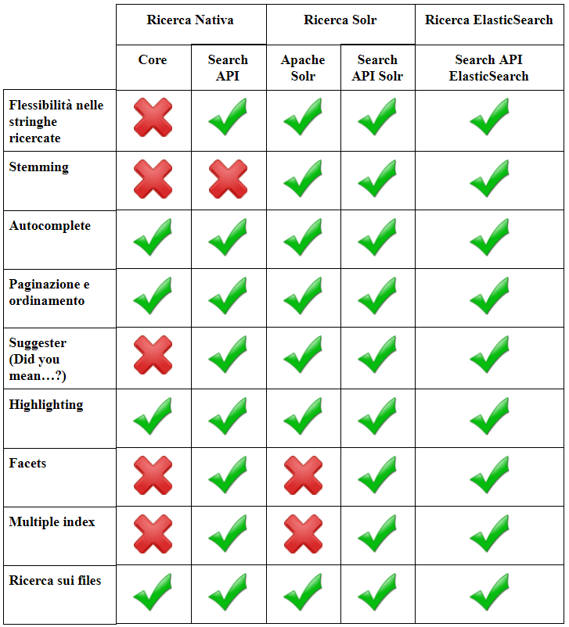
\includegraphics[width=1.3\linewidth]{confronto_finale}
		}
		\caption{Principali funzionalità di possibile interesse per i siti informativi Camerali e relativo supporto da parte dei motori di ricerca esaminati}
	\end{figure}		% Resoconto dello stage
	% !TEX root = ../../Tesi.tex

%******************************************
%	Valutazione retrospettiva
%******************************************

\chapter{Valutazione retrospettiva}
\label{valutazione_retrospettiva}

\section{Bilancio degli obiettivi}

	\subsection{Aziendali}
	
	Riprendendo gli obiettivi posti inizialmente dall'azienda riguardanti lo stage, presentati nella \hyperref[sub:obiettivi_posti_azienda]{sezione 2.2.2 : Obiettivi posti dall'azienda}, posso affermare di aver soddisfatto quanto mi era stato inizialmente richiesto. \\
	Le \gls{Milestone} previste sono infatti state raggiunte nei tempi prestabiliti, con un'eccezione: la presentazione dell'elaborato al team di lavoro, prevista per la fine dell'ottava settimana, è stata anticipata alla conclusione della settima settimana così da evitare l'incorrere di eventuali imprevisti. \\
	Nella prima settimana di lavoro, in aggiunta a quanto pianificato e su indicazione del tutor aziendale, ho studiato e configurato un \gls{Modulo} aggiuntivo dedicato alla ricerca che può essere considerato il passo intermedio tra quanto offerto nativamente dall'ambiente di sviluppo e i motori di ricerca più avanzati analizzati in seguito. Lo studio di tale modulo non ha comunque influito, a livello di tempistiche, su quanto pianificato per le settimane successive alla prima, ritrovandomi dunque allineato con quanto pianificato. \\
	Gli obiettivi aziendali, come già presentato nella \hyperref[subsub:priorita_degli_obiettivi_aziendali]{sezione 2.2.2, in concomitanza della "priorità degli obiettivi aziendali"}, sono stati suddivisi in due differenti tipologie: obiettivi minimi e massimi. \\
	Di seguito, riporterò una tabella nel quale viene indicato lo stato di superamento degli obiettivi dello stage a cui seguirà una specifica più dettagliata.

	\begin{longtable}{| C{2cm} | C{7cm} | C{2cm} |}
		\toprule
		\textbf{ID} & \textbf{Descrizione} & \textbf{Esito} \\ \hline
		\endhead	% Permette di ripetere l'intestazione nelle nuove pagine
		\midrule
		
		%%%%%	INIZIO BLOCCO FUNZIONALITA'	%%%%%
		
		\multicolumn{3}{|c|}{\cellcolor[HTML]{EFEFEF}\textbf{Obiettivi obbligatori (min) }} \\ \hline
		
		%%%%%	INIZIO BLOCCO TEST	%%%%%
		
		min01 &  Analisi dei punti di forza e debolezza dei prodotti \gls{Solr} ed \gls{ElasticSearch} & Soddisfatto \\ \hline
		
		%%%%%	FINE BLOCCO TEST	%%%%%
		
		%%%%%	INIZIO BLOCCO TEST	%%%%%
		
		min02 &  Realizzazione del prototipo in \gls{Drupal} con le funzioni minime di ricerca & Soddisfatto \\ \hline
		
		%%%%%	FINE BLOCCO TEST	%%%%%
		
		%%%%%	FINE BLOCCO FUNZIONALITA'	%%%%%
		
		
		
		%%%%%	INIZIO BLOCCO FUNZIONALITA'	%%%%%
		
		\multicolumn{3}{|c|}{\cellcolor[HTML]{EFEFEF}\textbf{Obiettivi desiderabili e opzionali (max) }} \\ \hline
		
		%%%%%	INIZIO BLOCCO TEST	%%%%%
		
		max01 & Comparazione dei due motori di ricerca esaminati con altri di riferimento nel mercato & Soddisfatto \\ \hline
		
		%%%%%	FINE BLOCCO TEST	%%%%%
		
		%%%%%	INIZIO BLOCCO TEST	%%%%%
		
		max02 &  Indicazioni su possibili interventi sui siti web istituzionali per quanto riguarda la user experience di navigazione, a seguito delle potenzialità espresse dai motori di ricerca & Soddisfatto \\ \hline
		
		%%%%%	FINE BLOCCO TEST	%%%%%
		
		%%%%%	FINE BLOCCO FUNZIONALITA'	%%%%%
		
		\bottomrule
		\caption{Superamento degli obiettivi dello stage}
	\end{longtable}

	\begin{itemize}
		
		\item {\textbf{[min01] Analisi dei punti di forza e debolezza dei prodotti \gls{Solr} ed \gls{ElasticSearch}}: Durante lo stage, ho avuto modo di esplorare le funzionalità offerte da queste due tecnologie, focalizzandomi su quelle di possibile interesse per l'azienda. Un confronto approfondito dei due motori di ricerca non si limiterebbe però alle funzionalità che ho analizzato. Le differenze di maggior rilievo emergono infatti studiandone l'aspetto sistemistico. Personalmente, ho avuto modo di esplorare una piccola parte della visione sistemistica fornita dalle due tecnologie, concentrandomi invece sulle richieste dell'azienda e quindi sullo studio delle funzionalità di possibile interesse per i siti informativi Camerali;}
		
		\item {\textbf{[min02] Realizzazione del prototipo in \gls{Drupal} con le funzioni minime di ricerca}: Per ogni tecnologia di ricerca analizzata ho creato un'istanza \gls{Drupal} ad essa dedicata, attraverso la quale ho verificato l'eventuale presenza delle funzionalità di possibile interesse per i siti informativi Camerali. Ho avuto inoltre modo di creare un prototipo che utilizzasse i dati e le configurazioni dell'attuale sito in produzione della Camera di Commercio di Verona, cambiandone la tecnologia di ricerca precedentemente utilizzata con il fine di migliorarne le funzionalità offerte;}
		
		\item {\textbf{[max01] Comparazione dei due motori di ricerca esaminati con altri di riferimento nel mercato}: Come spiegato nella \hyperref[sec:individuazione_dei_motori_di_ricerca]{Sezione 3.1 : Individuzione dei motori di ricerca}, sono state prese in considerazione ulteriori tecnologie di ricerca oltre a quelle esaminate;}
		
		\item {\textbf{[max02] Indicazioni su possibili interventi sui siti web istituzionali per quanto riguarda la user experience di navigazione, a seguito delle potenzialità espresse dai motori di ricerca}: Come evidenziato nella \hyperref[sub:possibile_evoluzione]{Sezione 3.3.2 : Possibile evoluzione}, ho proposto l'aggiunta di alcune funzionalità agli attuali siti informativi Camerali, prendendo come esempio l'attuale sito in produzione della Camera di Commercio di Verona (\cite{site:vr}), creandone un prototipo che utilizzasse le funzionalità proposte.}
		
	\end{itemize}

	A seguito del mio stage, l'azienda è stata inoltre in grado di ottenere alcuni risultati immediati:
	\begin{itemize}
		\item {La ricerca dei siti informativi delle Camere di Commercio di Bologna, Palermo-Enna e Sicilia Orientale ha visto un'evoluzione della tecnologia di ricerca utilizzata;}
		\item {E' stata migliorata la configurazione della ricerca del sito informativo della Camera di Commercio di Torino.}
	\end{itemize}

	\subsection{Personali}
	Lo stage svolto ha reso possibile la mia introduzione al mondo lavorativo in un'importante azienda che opera nel settore informatico. Nei due mesi trascorsi in \nomeAzienda, ho avuto l'opportunità di confrontarmi con personale qualificato, in possesso di un'ottica diversa da quella a cui sono abituato da studente universitario quale sono. Ho potuto applicare alcune delle conoscenze apprese durante il mio percorso di studi, evolvendo dalla mera conoscenza teorica ad una conoscenza pratica, certamente molto più richiesta e di interesse nell'attuale mercato del lavoro.
	
	\begin{itemize}
		
		\item {Motivazioni professionali: Come già affermato, lo stage in \nomeAzienda mi ha permesso di entrare in contatto con personale esperto e qualificato, che lavora nel mondo dell'informatica da anni, permettendomi così di espandere la mia rete di conoscenze di figure che operano nel mio stesso settore. Inoltre, ho potuto affinare le mie capacità di problem solving ed esplorare tecnologie attuali correlate ad un tema che ritengo di particolare interesse. Tutto ciò ha permesso di aumentare e migliorare le mie conoscenze e competenze, andando ad arricchire il mio curriculum professionale;}
		
		\item {Motivazioni economiche: L'azienda ha rispettato gli accordi inizialmente stabiliti, fornendomi un rimborso spese e buoni pasto;}
		
		\item {Motivazioni personali: Ho avuto modo di valutare se il percorso formativo da me scelto fosse quello corretto e se quanto fatto durante lo stage fosse realmente ciò a cui mi voglio dedicare nella vita.}
		
	\end{itemize}

\section{Conoscenze acquisite}
L'esperienza di stage in \nomeAzienda ha permesso di ampliare le mie conoscenze sia dal punto di vista organizzativo, sia da quello tecnologico. Più in dettaglio:

	\subsubsection{Conoscenze in ambito organizzativo}
	Come previsto inizialmente, l'attività di stage prevedeva incontri quotidiani con il tutor, in modo tale da risolvere eventuali dubbi o decidere di approfondire determinati ambiti di interesse. Così facendo, ho imparato a svolgere le attività programmate senza sprecare tempo su dettagli a volte irrilevanti. Eventuali problemi bloccanti, che non mi permettevano di procedere con il lavoro, sono stati tempestivamente risolti richiedendo l'intervento del tutor aziendale. Il numero di richieste è stato comunque limitato, in modo tale da non compromettere il lavoro e i progetti che il tutor aziendale stava seguendo. Così facendo, ho imparato a lavorare in autonomia, confrontandomi con personale più esperto solamente qualora lo ritenessi necessario.

	\subsubsection{Conoscenze in ambito tecnologico}
	Durante lo stage ho avuto modo di studiare ed esplorare nuove tecnologie; in particolare:
	\begin{itemize}
		\item[--] {ho avuto modo di conoscere e rapportarmi con un \gls{CMSg} (\gls{Drupal});}
		\item[--] {ho avuto modo di confrontarmi con query di un certo grado di complessità, per la comprensione di determinate funzionalità offerte dall'ambiente \gls{Drupal};}
		\item[--] {ho appreso il funzionamento di \gls{Acquia Dev Desktop 2}, rimanendo in ambito locale;}
		\item[--] {ho utilizzato il sistema \gls{Git} mediante un'interfaccia grafica in ambiente Windows;}
		\item[--] {ho avuto modo di conoscere ed utilizzare due tra i maggiori motori di ricerca \gls{open source} attualmente disponibili: \gls{Solr} ed \gls{ElasticSearch}.}
	\end{itemize}

\section{Mondo del lavoro e università a confronto}
L'esperienza di stage offre l'occasione di ampliare le conoscenze per lo più teoriche, apprese durante il percorso di studi, con conoscenze pratiche, ampiamente più richieste nell'attuale mondo del lavoro. Inoltre, rappresenta un'occasione che permette sia all'azienda, sia allo studente, di conoscersi  ed eventualmente di proseguire il rapporto lavorativo anche al termine dello stage. \\
Il ruolo dell'università dovrebbe consistere nel fornire allo studente le conoscenze di base per poter rendersi competitivo nel mercato del lavoro. Questo obiettivo risulta essere particolarmente ambizioso nell'ambito dell'informatica, data la rapida evoluzione delle tecnologie e le numerose aree di interesse che coinvolge. La natura mutevole delle tecnologie può suggerire che il miglior modo per affrontare questa situazione consista nell'impartire, durante i corsi universitari, conoscenze di base facilmente adattabili alle nuove tecnologie emergenti. \\
Focalizzando l'attenzione sull'esperienza di stage che ho svolto presso \nomeAzienda, reputo innanzitutto di fondamentale importanza le conoscenze apprese riguardanti l'organizzazione e i processi aziendali, che permettono allo studente di arrivare preparato in una realtà aziendale particolarmente strutturata, così com'è avvenuto nel mio specifico caso. I progetti e i lavori di gruppo, eventualmente corredati da presentazioni sul lavoro svolto, danno certamente un valore aggiunto al profilo dello studente. \\
Le tecnologie presentate nel corso degli studi universitari hanno reso possibile la facile comprensione delle tecnologie con le quali mi sono confrontato durante lo stage. \\
Al giorno d'oggi, sempre più aziende offrono lavoro in ambito web, esattamente com'è avvenuto nel mio caso. Personalmente, ritengo che uno studente laureato in Informatica, per potersi mettere in gioco nel mercato del lavoro, abbia la necessità di avere le basi necessarie ad affrontare i concetti legati ai \gls{CMSg}, e ai servizi \gls{REST}. Riterrei dunque opportuno approfondire queste tematiche in ambito universitario, organizzando ad esempio seminari che trattino questi argomenti. \\
In conclusione, ritengo l'esperienza di stage uno strumento molto utile e professionalizzante per lo studente, che va molte volte a colmare il gap presente tra il mondo accademico e il mondo del lavoro.		% Valutazione retrospettiva

	%******************************************
	% Parte finale
	%******************************************
	\backmatter
	\printglossaries
	
\end{document}